\documentclass[11pt]{article}
\usepackage{fontspec}
\setmainfont{Aptos}
\setmonofont{Hack}[Scale=0.85]
\usepackage{latexsym}
\usepackage[font=small,labelfont=bf]{caption}
\usepackage{booktabs}
\usepackage{tabto}
\usepackage{graphics}
\usepackage{array}
\usepackage{titlesec}
\usepackage{color,soul}
\usepackage[australian]{babel}
\usepackage[none]{hyphenat}         % Woordafbreking
\usepackage[left=2.50cm, right=2.50cm, top=3.00cm, bottom=3.00cm]{geometry} % Marges
\usepackage{parskip}                % Normale paragrafen
\usepackage[hidelinks]{hyperref}    % Klikbare verwijzingen                 
\usepackage{fancyhdr}               % Fancy headers
\usepackage{lastpage}               % Paginanummers in footer
\usepackage[english]{isodate}       % Normale datums
\usepackage{graphicx,ifthen}               % Plaatjes
\usepackage{float}                  % Whatever floats your goat
% textgreek not needed with fontspec/XeLaTeX — use Unicode Greek directly
\usepackage{mathtools}              % Gekke formules bouwe
\usepackage{doi}                    % DOIs linken
\usepackage{textcomp}               % Symbols (gensymb removed — incompatible with fontspec)
\usepackage[nottoc]{tocbibind}      % References in Table of contents
% Fonts set via fontspec above (Aptos 11pt, Courier New mono)
\frenchspacing                      % Normale spacing
\sloppy                             % Woordafbreking
\usepackage{listings}
\usepackage{color} %red, green, blue, yellow, cyan, magenta, black, white
\definecolor{mygreen}{RGB}{28,172,0} % color values Red, Green, Blue
\definecolor{mylilas}{RGB}{170,55,241}
\graphicspath{ {Figures/} }

% Word count — generated by: make wordcount (writes wordcount.tex)
% Fallback if file doesn't exist yet
\newcommand{\wordcount}{---}
\InputIfFileExists{wordcount.tex}{}{}

\usepackage[textsize=scriptsize]{todonotes}
\hypersetup{colorlinks=true,linkcolor=black,citecolor=blue!60!black,urlcolor=blue!60!black}
\usepackage{enumitem}
\usepackage{eurosym}
\usepackage[autostyle]{csquotes}
\usepackage{lscape}
%\usepackage[version=4]{mhchem}
\usepackage{booktabs}
\usepackage{amsmath}
\usepackage{amssymb}
\usepackage[style=authoryear,sorting=nyt,block=ragged,sortcites,giveninits,maxnames=4,backend=biber,dateabbrev=false,maxbibnames=99,uniquename=false,uniquelist=false]{biblatex}
\usepackage{csquotes}
% Make \cite produce parenthetical Harvard citations: (Author, Year)
\let\cite\parencite
% Hyperlink the entire citation, not just the year
\DeclareCiteCommand{\parencite}[\mkbibparens]
  {\usebibmacro{prenote}}
  {\bibhyperref{\usebibmacro{citeindex}%
   \usebibmacro{cite}}}
  {\multicitedelim}
  {\usebibmacro{postnote}}
\usepackage[normalem]{ulem}
\useunder{\uline}{\ul}{}
\numberwithin{equation}{section} 
\usepackage{chngcntr}
\counterwithin{figure}{section}
\counterwithin{table}{section}
%\newcommand*{\fullref}[1]{\hyperref[{#1}]{\autoref*{#1} \nameref*{#1}}}
\usepackage{tikz}
\usepackage{pgfplots}
\usepackage{pgfplotstable}
\pgfplotsset{compat=1.18}
\usetikzlibrary{arrows.meta,positioning,fit,decorations.pathreplacing,shapes.geometric}

% Colour cycle: TU Delft-inspired, accessible (used in benchmarks + diagrams)
\definecolor{plotblue}{HTML}{0077BB}
\definecolor{plotred}{HTML}{CC3311}
\definecolor{plotorange}{HTML}{EE7733}
\definecolor{plotcyan}{HTML}{009988}
\definecolor{plotgrey}{HTML}{888888}
\usepackage{url}
\usepackage{multirow}
\usepackage{tabulary}
\usepackage[titletoc,toc,page]{appendix}
\usepackage{subfig}
\usepackage{mdwlist}
\usepackage{pdfpages}
\urlstyle{same}
\titlespacing{\subsection}{0pt}{\parskip}{0.5\parskip}
\titlespacing{\subsubsection}{0pt}{\parskip}{0.25\parskip}
\captionsetup[table]{aboveskip=1pt,belowskip=6 pt}

\newcommand*{\BeginNoToc}{%
  \addtocontents{toc}{%
    \edef\protect\SavedTocDepth{\protect\the\protect\value{tocdepth}}%
  }%
  \addtocontents{toc}{%
    \protect\setcounter{tocdepth}{-10}%
  }%
}
\newcommand*{\EndNoToc}{%
  \addtocontents{toc}{%
    \protect\setcounter{tocdepth}{\protect\SavedTocDepth}%
  }%
}

\widowpenalties 1 10000	
\raggedbottom
%Bibliography
\addbibresource{main.bib}
% Render urldate as "accessed on <date>" instead of "visited on <date>"
\DeclareFieldFormat{urldate}{\mkbibparens{accessed on #1}}
\setlength{\bibitemsep}{0.5em}

\begin{document}

\pagenumbering{gobble}
% Cover sheet — required fields per Handbook 4.5.1 / 8.2.1
\begin{center}
\vspace*{-1cm}


\includegraphics[width=0.35\textwidth]{Figures/UniLogo.png}\\[1cm]

{\Large\bfseries Department of Computer Science}\\[0.5cm]
{\large BSc (Hons) Computer Science}\\[1.5cm]

{\LARGE\bfseries Lattice: Privacy-Preserving Sealed-Bid\\Auctions over Veilid with MPC}\\[1.5cm]

{\large Anker Rasmussen}\\[0.3cm]
{\small anker.rasmussen@city.ac.uk}\\[1cm]

{\large\textbf{Project Consultant:} Martin Brain}\\[0.3cm]
{\large\textbf{Client:} Martin Brain (Academic Client)}\\[1cm]

{\large\textbf{Category:} Academic Client Project}\\[0.3cm]
{\small\textbf{Subcategory:} Application Development}\\[1cm]

\textbf{Word count:} \wordcount{} / 12,000\\[0.3cm]
\textbf{Proprietary Interests:} None\\[0.3cm]
\textbf{Licence:} MPL-2.0

\vfill
\today
\end{center}


\newpage
% Abstract — 100-250 words (Handbook 8.1.1)
%
% === Questions for Martin (meeting notes) ===
%
% 1. Lead with privacy or engineering? The project is both a privacy system
%    and a hard engineering challenge (building on immature Veilid). Which
%    angle do markers care about more?
%
% 2. Seller-only-gets-a-route: the seller never learns the winner's identity
%    — just an ephemeral onion route. Stronger than most sealed-bid systems.
%    Worth emphasising in the abstract or too in-the-weeds?
%
% 3. Monero descope framing. Time went to MPC tunnel hardening + route
%    recovery + E2E tests instead. Was this the right tradeoff?
%
% 4. LSEPI / dual-use honesty level. The system *could* be deployed as a
%    real anonymous marketplace. The limitations (no Sybil resistance, seller
%    trust, liveness) are all fixable engineering problems, not fundamental.
%    How candid should the report be about this?
%
% 5. Assumptions up front vs in Results. Ch1 currently plans to state what
%    IS private, what ISN'T, trust assumptions, liveness constraints. Too
%    much for an intro, or good that markers see it immediately?
%
% 6. OT descope. PDD said 1-out-of-N OT for decryption key delivery.
%    Implemented commitment+challenge instead. Seller already sees winning
%    bid via MPC (party 0), so no additional info leak. Discuss as limitation
%    or pragmatic equivalent?
%
% ===========================================
\section*{Abstract}
\addcontentsline{toc}{section}{Abstract}

Bidder privacy is absent from mainstream online auctions.  Open-bid platforms
reveal the bidding process to all participants; sealed-bid schemes hide bid
values but still require a trusted auctioneer who sees every bid.  In both
models, losing bidders' information is unnecessarily exposed, and metadata ---
who bid, when, how often --- is visible to platform operators and network
observers.  This project explored whether a fully decentralised auction could
protect bidder privacy without any trusted intermediary.

A peer-to-peer sealed-bid marketplace was built on Veilid, a privacy-first
application framework providing onion-routed messaging, a secure distributed
hash table, and public-key identities with no central server.  Bids are
cryptographically committed and the winner is determined jointly by all
participants using the MASCOT multi-party computation protocol, so that losing
bid values are never revealed to anyone.  Network-level privacy is provided by
Veilid's private routing, which obscures participants' IP addresses and
locations.  Even the seller, who learns the winning bid value, receives only an
ephemeral onion route to the winner --- not their identity.

The prototype was implemented in Rust (approximately 14,800 lines of original
code) and tested on a 20-node devnet with automated end-to-end auction
scenarios.  A security analysis identified residual privacy limitations: bid
timing can leak party assignments, participation metadata is visible on the
DHT, and any single party going offline during MPC execution prevents the
auction from completing.


% Scope the definitions to be strict!
% Metadata about bids / What are you trying to protect, who are you trying to protect it from?`
\newpage
\section*{Acknowledgements}
\addcontentsline{toc}{section}{Acknowledgements}
I would like to thank my project consultant, Martin Brain, for his
outstanding support throughout this project.  Beyond setting a genuinely
interesting academic client project, he provided excellent ideas, discussed
architectural implementations in depth, and steered me away from rabbit
holes that would have consumed time and returned nothing.  His guidance
shaped the project at every stage.

I would also like to thank Christien Rioux (DilDog), lead developer of the
Veilid framework, and the Veilid Discord community.  The sheer volume of information available on the Discord, where other
developers had run into exactly the same issues and DilDog responded with
recommended architectural choices, accelerated development enormously and
directly informed the design of this system.
\newpage
\pagenumbering{roman}
\BeginNoToc
\listoffigures
\listoftables
% Glossary / Abbreviations — Handbook 8.2.8
\section*{Glossary}
\addcontentsline{toc}{section}{Glossary}

\begin{description}[style=nextline, labelwidth=5cm, leftmargin=5.5cm]

  % --- Standard CS (included because project-specific usage) ---
  \item[AES-256-GCM] Advanced Encryption Standard with 256-bit key in Galois/Counter Mode. An authenticated encryption scheme providing both confidentiality and integrity.
  \item[Commitment scheme] A two-phase cryptographic protocol: a party first publishes a binding commitment (e.g.\ a hash), then later reveals the committed value. Used here for sealed bids.
  \item[CRDT] Conflict-Free Replicated Data Type. A data structure designed for distributed systems where multiple nodes can update their own copy independently, and all copies are guaranteed to converge to the same state without coordination. Used in this project as a G-Set (grow-only set) for the bid announcement registry, ensuring that concurrent bid announcements from different nodes merge correctly without conflicts.
  \item[DHT] Distributed Hash Table. A decentralised key--value store where records are spread across participating nodes rather than held on a single server. Lookups are routed through the network so that no single node needs to store everything.
  \item[E2E] End-to-end. In this report, refers to tests exercising the full system stack including real Veilid networking.
  \item[NAT] Network Address Translation. Relevant because Veilid must traverse NATs (carrier-grade or regular) to establish peer connections.
  \item[P2P] Peer-to-Peer. A network model with no central server; all participants are equal.
  \item[SHA-256] Secure Hash Algorithm producing a 256-bit digest. Used for bid commitments: $C = \text{SHA-256}(\mathit{bid} \| \mathit{nonce})$.
  \item[TCP] Transmission Control Protocol. MP-SPDZ parties communicate over TCP; the MPC tunnel proxies TCP over Veilid.

  % --- MPC / Cryptography ---
  \item[Dishonest majority] An MPC security model tolerating corruption of up to $N{-}1$ of $N$ parties. Stronger than honest majority but more expensive. Used by MASCOT.
  \item[HE] Homomorphic Encryption. A form of encryption that allows mathematical operations to be performed on encrypted data without decrypting it first. The result, when decrypted, matches the outcome of performing the same operations on the plaintext. Used in some MPC protocols (e.g.\ the original SPDZ) as an alternative to oblivious transfer.
  \item[Honest majority] An MPC security model requiring that fewer than $N/2$ parties are corrupt. Used by Shamir secret sharing.
  \item[Integer triples] Pre-computed tuples $(a, b, c)$ where $c = a \cdot b$, shared among MPC parties. Also called Beaver triples. Used in SPDZ/MASCOT to reduce online multiplication to additions and openings, moving expensive computation to an offline preprocessing phase.
  \item[MAC] Message Authentication Code. In SPDZ/MASCOT, every secret-shared value carries a MAC tag under a global key ($\alpha$) that is itself secret-shared among all parties. When a value is opened, all parties verify the MAC; any tampering by a corrupt party causes the check to fail and the protocol to abort. This is what gives MASCOT its malicious security.
  \item[Malicious security] An MPC security model where corrupt parties may deviate arbitrarily from the protocol. Stronger than semi-honest security.
  \item[MASCOT] Malicious And Secure Computation using Oblivious Transfer. A dishonest-majority MPC protocol with malicious security~\cite{keller2016_mascot}.
  \item[MEV] Miner-Extractable Value. Profit that miners or validators can extract by reordering, inserting, or censoring transactions within a block before it is finalised. In the context of on-chain auctions, MEV enables front-running (seeing a pending bid and placing one's own bid ahead of it) and sandwich attacks (placing transactions both before and after a victim's transaction to artificially move the price and profit from the difference)~\cite{daian2019_flashboys2}.
  \item[MPC / SMPC] (Secure) Multi-Party Computation. Protocols enabling joint computation over private inputs without revealing them to other parties.
  \item[MP-SPDZ] Multi-Protocol SPDZ. A framework providing multiple MPC protocol backends from a single high-level program~\cite{mp-spdz}.
  \item[OT] Oblivious Transfer. A cryptographic primitive where a sender holds $N$ messages and a receiver selects one to receive. The sender learns nothing about which message was chosen, and the receiver learns nothing about the other messages. MASCOT uses OT extensively to generate the correlated randomness (integer triples) needed for secure multiplication.
  \item[Replicated secret sharing] The simplest multi-party MPC protocol, supporting exactly three parties. Each party holds two of the three shares of every secret value, so any two parties can reconstruct it. Requires an honest majority (at most one corrupt party). Used during early development as a ``hello world'' to validate the MPC integration pipeline.
  \item[Semi-honest security] An MPC security model assuming corrupt parties follow the protocol but try to learn extra information from intermediate values. Weaker than malicious security.
  \item[SPDZ] ``Speedz.'' A family of MPC protocols with dishonest-majority security, originally based on somewhat homomorphic encryption~\cite{damgaard2011_spdz}.
  \item[SSS] Shamir's Secret Sharing. A threshold scheme distributing a secret among $N$ parties such that any $t{+}1$ shares reconstruct it, but $t$ or fewer reveal nothing~\cite{shamir1979_secret_sharing}.
  \item[TEE] Trusted Execution Environment. A hardware-isolated processor region for secure computation. An alternative to MPC with different trust assumptions~\cite{li2023_secure_comp_tee_survey}.
  \item[Threshold cryptography] A cryptographic technique where a secret key is split among $N$ parties such that at least $t{+}1$ must cooperate to perform an operation (e.g.\ decryption or signing). No single party can act alone, removing single points of trust. Proposed as future work to eliminate the seller's exclusive control over decryption key release.

  % --- Veilid / Networking ---
  \item[\texttt{app\_call}] Veilid API for request--response messaging with confirmed delivery. Used for all reliable point-to-point communication in this system.
  \item[\texttt{app\_message}] Veilid API for fire-and-forget messaging without delivery confirmation. Used only for non-critical broadcasts.
  \item[I2P] Invisible Internet Project. An anonymity network similar to Tor but designed for internal (``darknet'') services rather than accessing the public internet. Uses garlic routing, a variant of onion routing that bundles multiple messages together for efficiency.
  \item[IPFS] InterPlanetary File System. A content-addressed P2P storage network with no built-in privacy layer.
  \item[Onion routing] A network anonymity technique where a message is encrypted in multiple layers (like the layers of an onion), one for each relay node on the path. Each relay strips one layer of encryption and forwards the result to the next hop. No single relay knows both the sender and the final destination, providing sender anonymity.
  \item[Overlay network] A virtual network built on top of physical infrastructure, where peers form logical links independent of their IP topology.
  \item[Private route] A Veilid construct: an onion-routed path through relay nodes, represented as an opaque blob that can be published and imported by remote peers.
  \item[Relay node] A peer in the Veilid overlay that forwards messages on behalf of other nodes without being the sender or final recipient. When a private route is constructed, it passes through one or more relay nodes; each relay strips a layer of encryption and forwards the result. The more relay nodes (hops) in a route, the harder it is to trace the message back to its origin, but each additional hop adds latency.
  \item[Hop] A single step in an onion-routed path. A message travelling through a private route with two hops passes through two relay nodes between sender and receiver. Veilid defaults to two hops per private route.
  \item[Route-in-DHT] A coordination pattern where a node writes its private route blob to a DHT record so that remote peers can discover and import it without direct messaging. Adapted from Stigmerge~\cite{stigmerge2024}.
  \item[Stigmergy] Indirect coordination through a shared environment rather than direct communication. The route-in-DHT pattern is an instance of stigmergy.
  \item[Tor] The Onion Router. An anonymity network using onion routing and exit nodes, designed for client--server communication rather than P2P.
  \item[Tunnelling] Encapsulating one protocol inside another to transport it across an intermediate network. Here: TCP-over-Veilid for MPC traffic.
  \item[Veilid] A privacy-first, open-source P2P application framework providing onion-routed messaging, a secure DHT, and pseudonymous public-key identities (no real names or IP addresses are exposed to other participants)~\cite{veilid_developer_book}.

  % --- Auction ---
  \item[English auction] An ascending-bid auction where the current highest bid is visible and bidders compete openly until no higher bid is placed.
  \item[First-price sealed-bid] An auction where bids are secret; the highest bidder wins and pays their bid price.
  \item[Front-running] An attack where an adversary observes a pending transaction (e.g.\ a bid) before it is finalised and submits their own transaction ahead of it to profit. In blockchain contexts, miners or validators can reorder transactions within a block to achieve this. See also MEV.
  \item[Sealed-bid auction] An auction where bids remain confidential during submission. Contrasts with open/English auctions.
  \item[Vickrey auction] A second-price sealed-bid auction: the highest bidder wins but pays the second-highest bid.

  % --- Tools / Formats ---
  \item[Bincode] A compact binary serialisation format. Used for ephemeral wire messages (\texttt{AuctionMessage} enum).
  \item[CBOR] Concise Binary Object Representation. A self-describing binary format used for DHT-stored records (listings, bids).
  \item[Dioxus] A React-inspired Rust framework for building cross-platform desktop applications (v0.7.2 used in this project).
  \item[Lattice] The peer-to-peer sealed-bid auction marketplace built in this project. Implemented in Rust, runs on the Veilid network, and uses MP-SPDZ for MPC-based winner determination.
  \item[LD\_PRELOAD] A Unix mechanism for intercepting library calls at runtime. Used here with \texttt{libipspoof.so} to give each Veilid node a unique public-facing IP address on a single machine. Veilid requires each node to appear as a distinct host on the public internet; without IP spoofing, multiple nodes on the same device fail to form separate routing identities.
  \item[MPL-2.0] Mozilla Public License 2.0. A file-level copyleft licence: modifications to MPL-licensed files must be published under MPL. Used by Veilid.

\end{description}

\EndNoToc
\newpage
\tableofcontents

\newpage
\pagenumbering{arabic}
% Chapter 1: Introduction — Handbook 8.2.2
% ~1000 words

\section{Introduction}
\label{sec:introduction}

\subsection{Problem Statement}
\label{sec:intro-problem}

Since the inception of the digital age, many established industries have moved
online.  Auction systems in particular have seen a massive surge in popularity
due to the low barrier to entry for both buyers and sellers: eBay sold
\$7.2~million worth of goods within a year of launch~\cite{ebay_history2025}
and today hosts 2.5~billion live listings across 135~million active
buyers worldwide~\cite{ebay_about2025}, and this is only one platform.  However, their
security models have not kept pace.  The move from physical sealed envelopes
to digital platforms introduced new attack surfaces, including bid visibility,
platform trust, and metadata exposure. Existing systems address
these concerns incompletely, if at all.

Popular online marketplaces follow three distinct patterns.  eBay uses open
proxy bidding: the current highest bid is visible throughout the auction and
the platform operator sees all bids~\cite{ebay_help_bidding}.  Facebook
Marketplace is a listing-plus-messaging workflow with no formal auction
protocol and weak buyer protections~\cite{fb_marketplace_help}.  Blockchain
marketplaces such as OpenSea~\cite{opensea2025} use English style auctions where
every bid is an on-chain transaction, publicly visible on all supported
chains~\cite{opensea_chains2025} and permanently recorded solving the
trusted-auctioneer problem via smart contracts, but providing zero bid privacy.

Government procurement offers a contrasting model.  Under the US Federal
Acquisition Regulation, sealed bidding keeps all bids confidential until a
public opening event~\cite{far_part14}.  Bids are private \emph{during}
submission, but a trusted auctioneer (the contracting officer) sees every bid
at opening and determines the winner.  Sealed bidding thus protects bids from
\emph{other bidders} but not from the \emph{auctioneer}.

Daian et al.\ demonstrated that even blockchain-based commit-reveal schemes
are vulnerable to front-running and miner-extractable value
(MEV)~\cite{daian2019_flashboys2}, where transaction ordering can be
exploited during the reveal phase.  Cryptographic sealed-bid auctions can
hide non-winning bids entirely~\cite{sako2000_hide_losers}, and multi-party
computation (MPC) can remove the need for a trusted auctioneer
altogether~\cite{bogetoft2009_mpc_live}.  However, deploying MPC over a
transport layer that also hides participants' network identities remains
largely unexplored.

\begin{table}[H]
\centering
\small
\renewcommand{\arraystretch}{1.3}
\makebox[\textwidth][c]{%
\begin{tabular}{|l|l|l|l|l|}
\hline
\textbf{System} & \textbf{Bids visible?} & \textbf{Trusted auctioneer?} & \textbf{Decentralised?} & \textbf{Bidder identity} \\
\hline
eBay              & Yes (open ascending) & Yes           & No  & Real name + address \\
\hline
OpenSea           & Yes (on-chain)       & No (contract) & Yes & Pseudonymous (wallet, IP visible) \\
\hline
US govt.\ sealed bid & No (until opening) & Yes (sees all)& No  & Real name (registered) \\
\hline
\textbf{Lattice(This project)} & \textbf{No (MPC)} & \textbf{No} & \textbf{Yes} & \textbf{Pseudonymous (key, IP hidden)} \\
\hline
\end{tabular}}%
\caption{Comparison of auction privacy models~\cite{ebay_help_bidding,opensea2025,far_part14}.}
\label{tab:auction-comparison}
\end{table}

\subsection{Security Policy}
\label{sec:intro-security-policy}

Privacy in this system meant protecting specific information from specific
adversaries.  Table~\ref{tab:security-policy-intro} summarises the security
policy; Chapter~\ref{sec:context} expands on the threat model in the context
of Veilid's network-layer protections.

\begin{table}[H]
\centering
\small
\renewcommand{\arraystretch}{1.3}
\makebox[\textwidth][c]{%
\begin{tabular}{|l|l|l|}
\hline
\textbf{What is protected} & \textbf{From whom} & \textbf{Mechanism} \\
\hline
Non-winning bid values & All parties (incl.\ seller) & MPC: only the maximum is revealed to party~0 \\
\hline
Bidder network identity (IP) & Network observers, other bidders & Veilid private routes (onion-routed, multi-hop) \\
\hline
Listing content before purchase & Non-winners & AES-256-GCM; key released only to verified winner \\
\hline
Bid existence and timing & Partially protected & DHT participation metadata remains visible \\
\hline
\end{tabular}}%
\caption{Security policy: what is protected and from whom.}
\label{tab:security-policy-intro}
\end{table}

The \emph{adversary model} considered four types, summarised in
Table~\ref{tab:adversary-model}.

\begin{table}[H]
\centering
\small
\renewcommand{\arraystretch}{1.3}
\makebox[\textwidth][c]{%
\begin{tabular}{|l|l|l|}
\hline
\textbf{Adversary} & \textbf{Capability} & \textbf{Goal} \\
\hline
Honest-but-curious bidder & Follows protocol, observes all available data & Learn other bids or bidder identities \\
\hline
Malicious seller & Controls listing, party~0 output, key release & Grief (withhold key), collude with preferred bidder \\
\hline
Passive network observer & Monitors DHT writes and message patterns & Deanonymise participants \\
\hline
Colluding parties & Multiple participants share private state & Break MPC threshold, reconstruct secret inputs \\
\hline
Dishonest participant & Participates in auction, observes protocol & Deanonymise other bidders or link pseudonyms to IPs \\
\hline
\end{tabular}}%
\caption{Adversary model.}
\label{tab:adversary-model}
\end{table}

Key \emph{trust and design assumptions}:

\begin{itemize}[noitemsep]
  \item The seller is semi-trusted: as MPC party~0 they learn the winning bid
    value and receive an ephemeral onion route to the winner, but not the
    winner's network identity.  The seller controls decryption key release
    and can grief by withholding the key.
  \item Veilid's private routing provides transport-layer anonymity; the
    effective anonymity set depends on both the number of relay nodes
    available in the overlay and the number of hops configured per
    private route. In this project's devnet; due to the devnet size, the hops default to 1.  More relay nodes increase the pool
    of possible intermediaries; more hops make traffic analysis harder
    but add latency per round trip.
  \item Liveness requires all MPC parties to remain online throughout
    computation.  A single party going offline aborts the auction.
  \item The MPC security guarantee depends on the protocol backend:
    MASCOT~\cite{keller2016_mascot} tolerates up to $N{-}1$ corrupt parties
    (dishonest majority)- and this is justified by the seller getting extra information in comparison to the bidding participants.
    Shamir~\cite{shamir1979_secret_sharing} requires
    an honest majority of at least $\lfloor N/2 \rfloor + 1$ honest parties.
  \item The system operates on a private devnet, not the public Veilid
    network.  All nodes are controlled by the tester; no real-world
    adversaries or network conditions are present or have been tested.
  \item Each Veilid node is assumed to have a unique public IP address.
    The devnet simulates this via LD\_PRELOAD IP spoofing
    (Section~\ref{sec:ctx-veilid-bootstrap}).
  \item Veilid supports only one active private route per node at a time.
    MPC sessions are therefore sequential; concurrent auctions on the same
    node are not possible.
  \item Party assignment is deterministic (sorted by bid timestamp).
    Any deterministic assignment from public data (timestamps, public keys,
    or otherwise) is publicly derivable and constitutes a known side channel.
    With MASCOT this is low severity, as the protocol is secure regardless
    of party identity; with Shamir it is more concerning if an attacker
    can target specific parties for corruption
    (Section~\ref{sec:results-security}).
  \item No Sybil resistance: Veilid itself provides no defence against
    a single adversary creating multiple pseudonymous identities.  By
    extension, nothing prevents one party from placing multiple bids in
    the same auction under different keys.  Mitigating this would require
    an identity layer that is out of scope.
  \item The auction is first-price only: the highest bidder wins and pays
    their bid. 
  \item No payment or settlement layer is integrated.  The auction ends
    at decryption key delivery; actual exchange of goods or funds is
    out of scope.
\end{itemize}

\subsection{Project Objectives}
\label{sec:intro-objectives}

The main objective was to deliver a working peer-to-peer marketplace on the
Veilid network supporting sealed-bid listings with private content unlock for
the winning bidder.  Four sub-objectives were defined in the PDD
(Appendix~\ref{app:pdd}):

\begin{enumerate}
  \item \textbf{Listings and purchases.}  End-to-end auction flow: create
    listing $\rightarrow$ submit bid $\rightarrow$ determine winner
    $\rightarrow$ complete purchase.
  \item \textbf{Sealed-bid via MPC.}  Integrate a multi-party computation
    protocol to select the highest valid bid without revealing non-winning bids.
  \item \textbf{MPC-gated decryption.}  Bind winner selection to content
    access: only the verified winner obtains the decryption key.
  \item \textbf{Settlement on Monero testnet.}  Simulate wallet
    initialisation, deposits, and release on a private Monero testnet.
    This objective was descoped as it was not inline with the research
    goals of the project, being more suited to a production system
    (Section~\ref{sec:conc-objectives}).
\end{enumerate}

\subsection{Beneficiaries}
\label{sec:intro-beneficiaries}

The project consultant gained a proof-of-concept demonstrating Veilid's
capabilities for a non-trivial use case.  The Veilid development community
benefited from a real application exercising the framework's private routing
and DHT APIs.  The project also contributed empirical data on the overhead of
tunnelling MPC through a privacy-preserving overlay. Also contributed was the 
playground infrastructure to the Veilid community; as a seperate testing environment
for users to test their own applications in a ``sandbox''.

\subsection{Report Structure}
\label{sec:intro-structure}

Chapter~\ref{sec:output-summary} summarises the deliverables.
Chapter~\ref{sec:context} provides technical background on the building
blocks: Veilid, MP-SPDZ, and the stigmerge coordination pattern, and expands
the security policy into a full threat model.
Chapter~\ref{sec:method} describes the architecture, protocol design, and
testing strategy.  Chapter~\ref{sec:results} presents verification:
functionality, performance benchmarks comparing MASCOT and Shamir over Veilid,
and a security analysis of residual information leakage.
Chapter~\ref{sec:conclusions} gives a critical overview, reflections, and
future work.


       % Ch 1: Introduction
% Chapter 2: Output Summary — Handbook 8.2.3
% Maximum 2 PAGES.

\section{Output Summary}
\label{sec:output-summary}

Table~\ref{tab:outputs} summarises the project deliverables.

\begin{table}[H]
\centering
\small
\renewcommand{\arraystretch}{1.3}
\makebox[\textwidth][c]{%
\begin{tabular}{|l|l|l|l|}
\hline
\textbf{Output} & \textbf{Type / Size} & \textbf{Recipient} & \textbf{Report reference} \\
\hline
Lattice application & Rust crate, ${\sim}$15k lines & Consultant, Veilid community & Sections~\ref{sec:results-architecture}--\ref{sec:results-testing} \\
\hline
\texttt{auction\_n.mpc} & MP-SPDZ DSL, 46 lines & Consultant & Section~\ref{sec:results-mpc} \\
\hline
Benchmark harness & Rust binary + 354 trials (CSV) & Consultant & Section~\ref{sec:results-benchmarks} \\
\hline
Devnet tooling & Makefile, playground orchestrator & Consultant, Veilid community & Section~\ref{sec:method-approach} \\
\hline
Demo video & 15-min narrated recording & Examiners & \textit{Submitted separately} \\
\hline
This report & LaTeX source in repo & Examiners & --- \\
\hline
\end{tabular}}%
\caption{Project deliverables.}
\label{tab:outputs}
\end{table}

The Lattice application was a desktop program built with Dioxus~0.7.2 that
embedded a Veilid node, provided a graphical interface for creating listings
and placing bids, and orchestrated the full MPC-based winner-determination
flow.  A headless binary (\texttt{market-headless}) was created to reduce the
friction of automated end-to-end testing without the overhead of running a GUI. 
The MPC protocol was drop-in: the auction
program compiled against any MP-SPDZ backend, and the runtime protocol was
selected via an environment variable.  MASCOT and Shamir were benchmarked,
but any MP-SPDZ protocol supporting $N$-party computation could be substituted
without code changes.

The benchmark harness (\texttt{bench-auction}) automated multi-party auction
trials across configurable party counts (3--20) and devnet sizes (40, 60, 80
nodes), collecting wall-clock time, MPC computation time, route-exchange
latency, tunnel bandwidth, and success rates.

\subsection*{Reuse Summary}

The application depended on Veilid (MPL-2.0) for networking, MP-SPDZ
(BSD-3-Clause) for MPC execution, and Dioxus (MIT/Apache-2.0) for the
desktop UI.  No code was directly copied from reference applications; the
\texttt{app\_call} delivery pattern over private routes was adapted from
Stigmerge~\cite{stigmerge2024}, a Veilid-based file-sharing application.
A detailed component-level reuse table is provided in Appendix~\ref{app:reuse}.

All source code, build scripts, benchmark data, and this report are available
in the project repository at
\url{https://github.com/anker-rasmussen/Dissertation} (including submodules).
The Rust crate was not published on crates.io or any public registry; it is
available only as source code in the repository.
      % Ch 2: Output Summary (max 2 pages)
% Chapter 3: Context — Handbook 8.2.4
% Literature review organised BY TOPIC, not by paper.
% ~1000 words for BSc. Cite everything. Show relevance to your project.

\section{Context}
\label{sec:context}

\subsection{Secure Multi-Party Computation}
\label{sec:ctx-mpc}

MPC enables a set of parties to jointly compute a function over their private
inputs without revealing those inputs to one
another~\cite{evans2018_pragmatic_mpc}.  The following definitions use the
formalisations in Evans et al.~(\citeyear{evans2018_pragmatic_mpc}) and
Zhao et al.~(\citeyear{zhao2019_secure_mpc}).  Two security models are central
to this project.

\subsubsection{Shamir Secret Sharing (Honest Majority)}
\label{sec:ctx-shamir}

Shamir's Secret Sharing~\cite{shamir1979_secret_sharing} hides a secret $s$
inside a random polynomial of degree $t$ whose constant term is $s$.  Each
party receives the polynomial evaluated at a distinct point.  Any $t{+}1$
parties can reconstruct $s$ via interpolation, but $t$ or fewer learn nothing
about it.

When used for MPC, the threshold is set to $t < N/2$ (honest majority).
Addition of shared values is free (each party adds its shares locally),
while multiplication requires one round of communication per gate, giving
$O(N)$ messages per multiplication.  This makes Shamir efficient at large
party counts.  However, if the honest-majority assumption is violated
($t \geq N/2$ parties are corrupt), the corrupt parties can reconstruct
every shared secret, and all privacy guarantees are lost.

\subsubsection{MASCOT (Dishonest Majority)}
\label{sec:ctx-mascot}

The MASCOT protocol~\cite{keller2016_mascot} is built on the SPDZ
framework~\cite{damgaard2011_spdz} and provides malicious security tolerating
up to $N{-}1$ corrupt parties.  The MPC program is expressed as an arithmetic
circuit: each operation (addition, multiplication, comparison) is a gate, and
the parties jointly evaluate the circuit by exchanging messages at each gate.
MASCOT operates in two phases.

\textbf{Offline phase (preprocessing).}  Before any inputs are known, the
parties generate a pool of authenticated Beaver triples using oblivious
transfer (OT).  For each pair of parties $(i, j)$, a series of OT instances
produces correlated random values that, when combined across all pairs, yield
a globally shared triple $(a, b, c)$ with $c = a \cdot b$.

Every shared value is authenticated with a MAC under a global key $\alpha$
that is itself secret-shared among all parties~\cite{damgaard2011_spdz}.
No single party knows $\alpha$, so no party can forge a valid share.

The pairwise nature of OT means the offline phase requires $O(N^2)$
communication: every pair of parties must exchange OT messages.  This is the
dominant cost and the reason MASCOT is significantly more expensive than
Shamir, particularly at higher party counts.

\textbf{Online phase (computation).}  Addition of shared values is free
(each party adds locally).  Multiplication consumes one pre-computed Beaver
triple per gate: the parties open masked values that reveal nothing about the
inputs, then combine the result with the triple to obtain a sharing of the
product.

The key difference from Shamir is what happens when a value is \emph{opened}
(revealed to all parties).  Before accepting an opened value $v$, all parties
perform a MAC check: each party $i$ computes $m_i - v \cdot \alpha_i$ and
the parties jointly verify that these sum to zero.  If any corrupt party
modified their share, the MAC check fails with overwhelming probability and
the protocol aborts.  This is what provides malicious security: corrupt
parties can deviate arbitrarily from the protocol, but any cheating is
detected before it affects the output.

A third protocol, replicated secret sharing, splits each secret into three
additive shares and gives each of the three parties two of them.  It is the
simplest multi-party scheme but is restricted to exactly three parties with an
honest majority.  It was used during early development to validate the MPC
integration pipeline before moving to MASCOT and Shamir for evaluation.

The MP-SPDZ framework~\cite{mp-spdz} provides academic production-grade
implementations of all three protocols, allowing the same high-level auction
program to be compiled and executed under different protocol backends.  This
was central to the evaluation in Chapter~\ref{sec:results}, where the same
program was benchmarked under MASCOT and Shamir with identical inputs.  Other
MP-SPDZ backends (semi-honest two-party, BMR garbled circuits, etc.) were not
tested because they either do not support $N > 2$ parties or solve a different
threat model than the one defined in Section~\ref{sec:intro-security-policy}.

The Danish sugar-beet auction~\cite{bogetoft2009_mpc_live} remains the most
prominent real-world MPC deployment for auctions, using a three-party
honest-majority protocol.  That system relied on a small number of known,
trusted intermediaries and a direct TCP network.  This project extended the
concept to an untrusted, peer-to-peer setting where the honest-majority
assumption may not hold, motivating the comparison between MASCOT and Shamir.

Zhao et al.~\cite{zhao2019_secure_mpc} survey MPC theory and applications.
Feng and Yang~\cite{feng2022_concretely_efficient_mpc} provide concrete
efficiency benchmarks, noting that the choice between honest and dishonest
majority remains the dominant factor in practical performance.  Li et
al.~\cite{li2023_secure_comp_tee_survey} compare MPC with trusted execution
environments (TEEs), concluding that MPC provides stronger trust assumptions
at the cost of higher communication overhead.

\subsection{Veilid: Privacy-Preserving Peer-to-Peer Networking}
\label{sec:ctx-veilid}

Veilid is described by its developers as
\begin{quote}
``an open-source, peer-to-peer application framework designed to build
privacy for all''~\cite{veilid_website}.
\end{quote}
Each application embeds a Veilid node into a global overlay where peers are
equal (no privileged relays), connections are end-to-end encrypted, and
private routing obscures network locations.

Three capabilities made Veilid suitable for this project:
\begin{enumerate}[noitemsep]
  \item \textbf{Addressable encrypted endpoints} keyed by public keys rather
    than IP addresses, eliminating direct IP exposure.
  \item \textbf{A secure DHT} for publishing listings, bids, and discovering
    auction participants.
  \item \textbf{Onion-routed private routes} for point-to-point messaging
    that limit metadata exposure during bid submission and MPC tunnel traffic.
\end{enumerate}

\subsubsection{What Veilid Protects (and What It Does Not)}
\label{sec:ctx-veilid-security}

Veilid's private routes provide network-layer anonymity: a sender constructs
a multi-hop route through relay nodes, and the receiver sees only the last
hop's identity.  This protects participants' IP addresses from each other and
from passive network observers.  However, several limitations were relevant to
the security policy:

\begin{itemize}[noitemsep]
  \item \textbf{Anonymity set}: Privacy depends on the number of available
    relay nodes.  On a small devnet (20--80 nodes), the anonymity set is
    correspondingly small.  On the public Veilid network this would be larger
    but remains unquantified.
  \item \textbf{DHT metadata}: Writing a bid record to the DHT is observable
    by DHT nodes.  The \emph{number} and \emph{timing} of bids are visible
    even though \emph{values} are encrypted.
  \item \textbf{Route liveness}: Private routes are application-managed and
    can die silently.  There is no notification when a remote route becomes
    invalid; sending to a dead route fails only after a timeout.  This had
    significant implications for MPC integration
    (Section~\ref{sec:results-mpc}).
  \item \textbf{IP leakage without private routes}: If a node communicates
    using unsafe routing (direct node-to-node), its IP address is exposed on
    the wire.  All benchmarked messaging in this system used safe routing
    exclusively.
\end{itemize}

Table~\ref{tab:overlay-comparison} compares Veilid with three alternative
overlay networks that offer similar privacy properties.

\begin{table}[H]
\centering
\small
\renewcommand{\arraystretch}{1.3}
\makebox[\textwidth][c]{%
\begin{tabular}{|l|l|l|l|l|}
\hline
\textbf{Property} & \textbf{Tor} & \textbf{I2P} & \textbf{IPFS} & \textbf{Veilid} \\
\hline
Primary model     & Client--server (exit nodes) & Internal services & Content-addressed storage & P2P application framework \\
\hline
Anonymity routing & Onion circuits (3 hops)     & Garlic routing     & None (cleartext DHT)      & Onion-routed private routes \\
\hline
Built-in DHT      & Hidden-service descriptors  & LeaseSet/NetDB     & Content routing            & General-purpose key--value \\
\hline
Embeddable library & No (SOCKS proxy)           & Partial (I2CP)     & Yes (libp2p)               & Yes (veilid-core) \\
\hline
P2P messaging     & Via hidden services         & Via streaming lib   & No                         & \texttt{app\_call} / \texttt{app\_message} \\
\hline
\end{tabular}}%
\caption{Overlay network comparison.}
\label{tab:overlay-comparison}
\end{table}

Tor~\cite{dingledine2004_tor} provides strong anonymity through onion-routed
circuits but is designed for the client--server model: clients reach clearnet
servers via exit nodes, or hidden services via rendezvous points.  Building a
peer-to-peer auction on Tor would require running each participant as a hidden
service, managing circuit lifecycle externally, and implementing DHT storage
separately.  Tor's hidden services also impose a minimum of six hops per
connection (three per side), adding latency that compounds across MPC rounds.

I2P~\cite{zantout2011_i2p} is closer to a P2P model, using garlic routing to
bundle messages for internal (``eepsite'') services.  Its streaming library
supports bidirectional TCP-like connections between I2P destinations.  However,
I2P lacks a general-purpose DHT for application data (its NetDB stores only
router and destination metadata), and its ecosystem is smaller with fewer
maintained client libraries.

IPFS~\cite{benet2014_ipfs} provides content-addressed storage over a
Kademlia-based DHT and is well suited for data distribution.  However, it
provides no anonymity: DHT operations and data transfers expose participants'
IP addresses.  Adding a privacy layer would require tunnelling IPFS through Tor
or I2P, combining the limitations of both.

Veilid was selected because it provides all three capabilities required by the
application in a single embeddable library: a general-purpose DHT for
storing listings and bids, onion-routed private routes for anonymous messaging,
and a peer-to-peer architecture where all nodes are equal with no privileged
relays or exit nodes.  This avoided the need to compose multiple
frameworks (e.g.\ IPFS for storage plus Tor for anonymity) and the integration
complexity that would entail.

\subsubsection{Bootstrap and Network Formation}
\label{sec:ctx-veilid-bootstrap}

A Veilid network requires at least one \emph{bootstrap node}: a
well-known server whose address is configured into every joining node so
that they can discover initial peers and populate their routing
tables~\cite{veilid_bootstrap_setup}.  On the public Veilid network,
bootstrap nodes are discovered via DNS TXT records.  For development and
testing, a private devnet must provide its own bootstrap infrastructure.

Crucially, Veilid expects each node to present a unique public IP address.
Its routing-domain logic classifies incoming connections by IP range and
drops traffic from addresses it considers local or
duplicate~\cite{veilid_developer_book}. Veilid also implements its own STUN for nodes
behind some level of NAT, but nodes behind NAT are not deemed ``optimal'', and recieve
network connection penalties accordingly (cannot act as bootstrap/less priority for relay).
This means that running multiple nodes on a single machine as required for a local devnet fails
unless each node appears to be on the public internet and not behind a NAT layer.  A community-contributed development
network~\cite{veilid-devnet-mr444} uses Docker containers with
per-container IP addresses.  This project's playground devnet took a lighter
approach: \texttt{LD\_PRELOAD} IP spoofing via a shared library
(\texttt{libipspoof.so}) that intercepts socket calls and maps each process to
a unique fake global IP (e.g.\ \texttt{1.2.3.1} through \texttt{1.2.3.255}),
supporting up to 255 nodes on a single machine without containerisation.
The implications of this constraint for devnet design are discussed further in
Section~\ref{sec:method-approach}.

\subsection{Stigmerge and the Route-in-DHT Pattern}
\label{sec:ctx-stigmerge}

Stigmerge~\cite{stigmerge2024} is a decentralised file-sharing application
built on Veilid that demonstrated the coordination patterns this project
adapted.  The name refers to \emph{stigmergy},indirect coordination through
a shared environment,where peers communicate by reading and writing shared
DHT records rather than maintaining direct connections.

Stigmerge established two patterns adopted in this project:
\begin{enumerate}[noitemsep]
  \item \textbf{Route-in-DHT}: A node creates a private route, serialises the
    route blob, and writes it to a DHT subkey.  Remote peers read the subkey,
    import the blob, and send messages via \texttt{app\_call} to the imported
    route.  This decouples route exchange from direct messaging.
  \item \textbf{\texttt{app\_call} for confirmed delivery}: All point-to-point
    data transfer uses Veilid's \texttt{app\_call} (request--response/SYN \& ACK) rather
    than \texttt{app\_message} (fire-and-forget), ensuring that failed
    deliveries are detected immediately rather than silently dropped.
\end{enumerate}

These patterns were critical for MPC tunnelling, where every message had to be
confirmed and route failures had to be detected promptly.

\subsection{Auction Privacy in Context}
\label{sec:ctx-auction-privacy}

Sako~\cite{sako2000_hide_losers} was the first to propose a cryptographic
auction protocol in which losing bids are never revealed.  The scheme uses
homomorphic encryption and zero-knowledge proofs so that the auctioneer can
publicly verify that the announced winner holds the highest bid, without
disclosing the values submitted by any other participant.  Sako proved the
protocol's correctness and privacy properties formally but did not produce an
implementation, leaving practical feasibility as an open question.
Blockchain-based auctions remove
the trusted auctioneer via smart contracts but expose all bids on-chain and
invite front-running~\cite{daian2019_flashboys2}.  The Danish sugar-beet
auction~\cite{bogetoft2009_mpc_live} demonstrated MPC in production but relied
on three trusted intermediaries operating over direct TCP.

This project combined the privacy guarantees of MPC (non-winning bids never
revealed) with the transport-layer anonymity of Veilid (participant IPs never
exposed), in a fully decentralised setting with no trusted auctioneer.

The seller occupies a semi-trusted role as MPC party~0.  This is justified
on two grounds.  First, the seller has a direct economic incentive to complete
the auction honestly: withholding the decryption key or manipulating results
means the sale does not proceed, costing the seller revenue.  Second, the
seller is the inherent key holder: since they encrypted the listing content,
they necessarily possess the decryption key, and any scheme that removes
the seller from key delivery requires threshold cryptography
(Section~\ref{sec:conc-future}).  The seller's power is strictly limited
ephemeral route to the winner, not all bids or bidder identities.

Chapter~\ref{sec:results} evaluates the cost of this combination in terms of
performance overhead, reliability, and residual information leakage.


%% TODO: Architecture diagrams for Ch5 (sequence, module dependency)            % Ch 3: Context / Literature Review (~1000w)
\include{Ch4_Method}             % Ch 4: Method (~2500w)
% Chapter 5: Results — Handbook 8.2.6
% ~6000 words

\section{Results}
\label{sec:results}

This chapter presents the evidence that the system works, how well it performs,
and what privacy it actually provides.  Each section ties back to the security
policy defined in Section~\ref{sec:intro-security-policy}.

\subsection{System Architecture}
\label{sec:results-architecture}

The final system had four layers: a Dioxus desktop UI (with a headless
binary for testing), an auction coordination layer (state machine, DHT
operations, MPC orchestration), the MPC tunnel proxy (bridging MP-SPDZ's
TCP to Veilid \texttt{app\_call}), and the Veilid overlay (DHT, private
routes, node identity).  There was no central server and no direct IP
connections between participants.  All persistent state was CBOR-serialised
into DHT records and all real-time communication travelled over
onion-encrypted private routes.

\subsubsection{DHT as Shared State}

The marketplace is bootstrapped from a single shared DHT record: the
\emph{master registry}.  All Lattice nodes know this record's key (derived
from the network key) and share a write keypair, so any node can add entries.
The full record hierarchy is shown in Figure~\ref{fig:dht-hierarchy}.

The DHT lifecycle (seller registration, listing creation, discovery, bidding,
and MPC route exchange) follows the record hierarchy in
Figure~\ref{fig:dht-hierarchy}.  The master registry and bid announcement
registries use a G-Set CRDT: each write merges the local set with the DHT
value via commutative union, so all nodes converge regardless of write order.

\subsection{Auction Protocol}
\label{sec:results-protocol}

The auction lifecycle, following the state machine in
Figure~\ref{fig:auction-fsm}, proceeds in seven phases:

\begin{enumerate}
  \item \textbf{Listing creation.}  The seller generates an AES-256-GCM key,
    encrypts the listing content, publishes the listing record to the DHT,
    and announces the listing key via broadcast \texttt{app\_message} to
    registered peers.

  \item \textbf{Bid submission.}  Each bidder creates a commitment
    $C = \text{SHA-256}(\mathit{bid} \| \mathit{nonce})$ with a
    cryptographically random 32-byte nonce, writes a bid record to the DHT,
    and announces the bid key to the listing's announcement registry.  The
    seller's node automatically places an auto-bid at the reserve price
    (party~0).

  \item \textbf{Deadline and party assignment.}  When the listing deadline
    expires, all nodes independently compute the same party assignment by
    sorting bidders by timestamp ascending (the seller's auto-bid is always
    earliest, becoming party~0).  This deterministic assignment requires no
    coordination.

  \item \textbf{MPC route exchange.}  Each party creates a Veilid private
    route and writes the route blob to their bid record's subkey~1.  Parties
    discover each other's routes via DHT reads with \texttt{app\_message}
    announcements as a fast path.  A readiness barrier
    (\texttt{MpcReady} via \texttt{app\_call}) ensures all routes are live
    before proceeding.

  \item \textbf{MPC execution.}  The \texttt{MpcOrchestrator} launches a
    local \texttt{mascot-party.x} (or \texttt{shamir-party.x}) process,
    feeds each party's bid value as secret input, and tunnels all inter-party
    TCP traffic through the Veilid \texttt{app\_call} tunnel.  The MPC
    program (Listing~\ref{lst:auction-mpc}) computes the maximum bid and
    reveals the winner ID and winning bid value only to party~0.

  \item \textbf{Winner verification.}  The seller sends a challenge to the
    claimed winner via \texttt{app\_call}.  The winner responds with their
    bid value and nonce; the seller verifies that
    $\text{SHA-256}(\mathit{bid} \| \mathit{nonce}) = C$.

  \item \textbf{Decryption key transfer.}  Upon successful verification, the
    seller sends the AES-256-GCM decryption key to the winner via
    \texttt{app\_call}.
\end{enumerate}


\begin{figure}[htbp]
\begin{lstlisting}[language=Python,basicstyle=\small\ttfamily,numbers=left,
  numberstyle=\tiny\color{gray},frame=single,xleftmargin=2em]
# n-Party Sealed-Bid Auction (First-Price)
# Party 0 = seller (reserve price). Parties 1..N = bidders.

n_parties = int(program.args[1])

# Each party inputs their bid as a secret integer
bids = Array(n_parties, sint)
for i in range(n_parties):
    bids[i] = sint.get_input_from(i)

# Find maximum bid and winner
max_bid = bids[0]
winner = sint(0)
for i in range(1, n_parties):
    is_higher = bids[i] > max_bid
    max_bid = is_higher.if_else(bids[i], max_bid)
    winner = is_higher.if_else(sint(i), winner)

# Reveal winner and bid ONLY to party 0 (seller)
winner_id = winner.reveal_to(0)
winning_bid = max_bid.reveal_to(0)
print_ln_to(0, 'Winner: Party %s', winner_id)
print_ln_to(0, 'Winning bid: %s', winning_bid)

# Each other party learns only won/lost
for party in range(n_parties):
    am_i_winner = (winner == sint(party)).reveal_to(party)
    print_ln_to(party, 'You won: %s', am_i_winner)
\end{lstlisting}
\caption{The MPC auction program (\texttt{auction\_n.mpc}), written in the
  MP-SPDZ DSL.  The comparison on line~16 and conditional select on lines
  17--18 are computed over secret-shared values - \(sint\), the provided primitive 
  for an (appropriately named) secret int within SPDZ. No party sees intermediate results. 
  The \texttt{reveal\_to(0)} calls on lines~21--22 ensure that
  only party~0 (the seller) learns the winner identity and winning bid.}
\label{lst:auction-mpc}
\end{figure}

\subsection{MPC Integration}
\label{sec:results-mpc}

\subsubsection{The Auction Program}

The \texttt{auction\_n.mpc} program (46 lines) implemented a first-price
sealed-bid auction for $N$ parties.  Each party inputs their bid as a secret
integer; the program computes the maximum and reveals (i)~the winner identity
and winning bid to party~0 only, and (ii)~a binary ``won: 0/1'' to each other
party.  The program is compiled once and executed with the appropriate party
count flag (\texttt{-N}). Note that for honest majority protocols executed within SPDZ, OpenSSL certificates
are required to be generated at compile time for each potential participant, and shared before the MPC reaches runtime. 
This is an advantage of using a dishonest majority protocol; no SSL secret shares prior to executing the MPC.

\subsubsection{Tunnel Architecture}

The MPC tunnel sent TCP over Veilid private routes.  Outgoing and incoming
traffic each ran in its own async task.  Sends were pipelined (up to eight
\texttt{app\_call} requests in flight at once) to minimize network latency.
The receiver reassembled the byte stream using sequence numbers and a reorder
buffer, since Veilid does not guarantee ordered delivery. Veilid has a limit of 32KB payloads
per communication envelope, and so the app\_calls were maxsized at 32KB each.

Table~\ref{tab:tunnel-volumes} shows the data volumes per protocol and party
count.  MASCOT's pairwise OT produces two to three orders of magnitude more
tunnel traffic than Shamir, meaning more \texttt{app\_call} round trips and
longer wall-clock times.

\begin{table}[H]
\centering
\small
\begin{tabular}{lrrrr}
\toprule
\textbf{Protocol} & $N$ & \textbf{Per-party (MB)} & \textbf{Total (MB)} &
  \textbf{App\_calls} \\
\midrule
MASCOT & $3$  & 37   & 107   & 3,416 \\
MASCOT & $6$  & 209  & 1,192 & 38,165 \\
MASCOT & $10$ & 653  & 6,213 & 198,747 \\
\midrule
Shamir & $3$  & 0.02  & 0.11  & 4 \\
Shamir & $6$  & 0.21  & 1.2   & 39 \\
Shamir & $10$ & 0.61  & 4.2   & 134 \\
Shamir & $20$ & 2.5   & 25.6  & 842 \\
\bottomrule
\end{tabular}
\caption{Data volumes tunnelled through Veilid per auction.  Each
  \texttt{app\_call} carries up to 32\,KB of payload.  MASCOT transfers
  roughly 1,000$\times$ more data than Shamir at $N{=}3$, growing to
  1,500$\times$ at $N{=}10$ due to $O(N^2)$ pairwise OT.}
\label{tab:tunnel-volumes}
\end{table}

\subsubsection{Route Lifecycle Challenges}

Veilid private routes are the single largest source of engineering complexity
in the system.  Three problems were encountered and solved:

\begin{enumerate}
  \item \textbf{Silent death.}  Routes die without notification; the only
    signal is a timeout on the next \texttt{app\_call}.  The system implemented
    reactive route refresh: if the readiness barrier detected fewer successful
    acknowledgements than expected, the node recreated its route, republished
    to the DHT, and polled peers' DHT entries for updated blobs.

  \item \textbf{Single active route.}  Veilid supports only one active
    private route per node.  Creating a second route invalidates the first.
    This means MPC sessions must be sequential, never concurrent.  When
    multiple auctions expire simultaneously, expired listings are sorted
    deterministically by key to ensure all nodes process them in the same
    order.

  \item \textbf{Self-import requirement.}  After creating a private route
    via \texttt{new\_private\_route()}, the node must call
    \texttt{import\_remote\_private\_route()} on its own blob.  Without this
    step, only one of $N$ created routes is deliverable.  This behaviour is
    undocumented but was confirmed by the Veilid core developers.
\end{enumerate}

These workarounds add approximately 200 lines of code.  Veilid~0.6.0 will
introduce DHT-published route blobs that are automatically fetched and
imported on use, eliminating the need for manual route
management~\cite{rioux2025_dht_patterns}.

\subsection{User Interface}
\label{sec:results-ui}

The Dioxus desktop application provided four main views: a marketplace
browser showing active listings, a listing creation form with deadline and
reserve price fields, a bid placement dialog, and an auction results view
showing the winner notification or decryption key.  The UI communicated with
the auction coordination layer through shared \texttt{Arc<Mutex<AppState>{}>}
state, polled by the Dioxus render loop.

The UI was not a focus of the project; it served as a thin presentation layer
demonstrating that the underlying protocol is usable interactively.  A
separate headless binary (\texttt{market-headless}) provided the same auction
logic without the UI, enabling automated E2E testing and benchmarking.  The
headless binary accepts listing parameters, bid values, and deadlines via
command-line arguments and environment variables, writes structured output
(JSON events) to stdout, and exits after the auction completes or times out.

\subsection{Testing and Verification}
\label{sec:results-testing}

\subsubsection{Test Coverage}

Table~\ref{tab:test-matrix} summarises the test suite.

\begin{table}[H]
\centering
\small
\begin{tabular}{llrl}
\toprule
\textbf{Level} & \textbf{Scope} & \textbf{Count} & \textbf{Runtime} \\
\midrule
Unit        & Modules (traits, serialisation, crypto) & 169 & $< 1$\,s \\
Integration & Full $N$-party auctions (mock DHT)      & 63  & $< 1$\,s \\
E2E         & Playground devnet, real Veilid networking & 3           & 3--8\,min each \\
\bottomrule
\end{tabular}
\caption{Test matrix.}
\label{tab:test-matrix}
\end{table}

\subsubsection{Integration Test Results}

The mock-based integration tests exercise the auction state machine with
3, 5, and 10 parties, covering:
\begin{itemize}[noitemsep]
  \item Highest bid wins and receives decryption key.
  \item Tied bids resolved by earliest timestamp.
  \item Reserve price enforced (auto-bid wins if no bidder exceeds it).
  \item Expired listings detected and processed.
  \item Commitment verification rejects incorrect nonces.
\end{itemize}

All 232 tests (unit + integration) pass consistently with zero flakiness.

\subsubsection{End-to-End Test Results}

The three E2E tests ran against a 20-node playground devnet:

\begin{itemize}[noitemsep]
  \item \textbf{Happy path} (169\,s): single 3-party auction
    completes successfully, winner receives decryption key.
  \item \textbf{Sequential} (380\,s): two auctions in sequence;
    tests route refresh between sessions.
  \item \textbf{Concurrent} (284\,s): two auctions with overlapping
    deadlines; verifies deterministic ordering prevents deadlock.
\end{itemize}

All three tests pass reliably on a clean devnet.  The devnet must be
restarted between test runs because Veilid's routing tables retain stale
entries for nodes that no longer exist; reconnecting on the same IP triggers
a one-hour penalty before the node is accepted again.  Additionally,
reconnecting with a different node identity on the same IP forces peers to
flush their cached knowledge of the previous node, and Veilid nodes
generally reject multiple node identities from a single IP address.

\subsection{Performance Benchmarks}
\label{sec:results-benchmarks}

The benchmark harness ran each configuration 5 times across three devnet
sizes (40, 60, 80 nodes), with party counts from 3 to 20.  Benchmarks were
run across two machines and results were combined:

\begin{itemize}[noitemsep]
  \item \textbf{Laptop}: AMD Ryzen AI 5 340 (12 cores) @ 4.90\,GHz,
    32\,GB DDR5, Arch Linux.
  \item \textbf{Desktop}: AMD Ryzen 7 5800X (16 threads) @ 4.85\,GHz,
    32\,GB DDR4, Arch Linux.
\end{itemize}

Figures in this section are generated from 354 trial rows
(153 direct TCP, 201 over Veilid).

% Benchmark figures for Chapter 5 — Performance Results
% Generated from bench-results/ CSVs via scripts/preprocess_benchmarks.py
% Re-run the script after adding new data, then recompile.

% Colours defined in Dissertation.tex preamble (plotblue, plotred, etc.)

\pgfplotsset{
  bench base/.style={
    width=0.88\columnwidth,
    height=6.5cm,
    grid=major,
    grid style={gray!30},
    tick label style={font=\small},
    label style={font=\small},
    legend style={font=\footnotesize, draw=none, fill=white, fill opacity=0.8},
    every axis plot/.append style={thick, mark size=2pt},
  },
}

%% ----------------------------------------------------------------
%% Figure 1: Direct MPC baseline (no Veilid)
%% ----------------------------------------------------------------
\begin{figure}[htbp]
  \centering
  \begin{tikzpicture}
    \begin{axis}[
      bench base,
      xlabel={Number of parties ($N$)},
      ylabel={Wall-clock time (s)},
      ymode=log,
      log basis y=10,
      xtick={3,4,5,6,8,10,15,20},
      legend pos=north west,
    ]
    \addplot+[color=plotred, mark=square*,
      error bars/.cd, y dir=both, y explicit]
      table[x=parties, y=wall_median, y error=wall_stddev]
      {Figures/data/direct_mascot.dat};
    \addlegendentry{MASCOT}

    \addplot+[color=plotblue, mark=triangle*,
      error bars/.cd, y dir=both, y explicit]
      table[x=parties, y=wall_median, y error=wall_stddev]
      {Figures/data/direct_shamir.dat};
    \addlegendentry{Shamir}

    \addplot+[color=plotgrey, mark=diamond*, only marks, mark size=3pt]
      table[x=parties, y=wall_median]
      {Figures/data/direct_rep-ring.dat};
    \addlegendentry{Rep-ring ($N{=}3$ only)}
    \end{axis}
  \end{tikzpicture}
  \caption{Direct MPC computation time (localhost TCP, no Veilid overlay).
    MASCOT scales quadratically with party count due to pairwise OT setup;
    Shamir scales linearly.  Error bars show $\pm 1$ standard deviation
    over 10 iterations.}
  \label{fig:direct-mpc-baseline}
\end{figure}

%% ----------------------------------------------------------------
%% Figure 2: Veilid auction total time — MASCOT
%% ----------------------------------------------------------------
\begin{figure}[htbp]
  \centering
  \begin{tikzpicture}
    \begin{axis}[
      bench base,
      xlabel={Number of parties ($N$)},
      ylabel={Total auction time (s)},
      xtick={3,4,5,6,8,10,12},
      legend pos=north west,
      ymin=0,
    ]
    \addplot+[color=plotblue, mark=*,
      error bars/.cd, y dir=both, y explicit]
      table[x=parties, y=total_median, y error=total_stddev,
            restrict expr to domain={\thisrow{n_success}}{1:99}]
      {Figures/data/veilid_mascot_40.dat};
    \addlegendentry{40-node devnet}

    \addplot+[color=plotorange, mark=square*,
      error bars/.cd, y dir=both, y explicit]
      table[x=parties, y=total_median, y error=total_stddev,
            restrict expr to domain={\thisrow{n_success}}{1:99}]
      {Figures/data/veilid_mascot_60.dat};
    \addlegendentry{60-node devnet}

    \addplot+[color=plotred, mark=triangle*,
      error bars/.cd, y dir=both, y explicit]
      table[x=parties, y=total_median, y error=total_stddev,
            restrict expr to domain={\thisrow{n_success}}{1:99}]
      {Figures/data/veilid_mascot_80.dat};
    \addlegendentry{80-node devnet}
    \end{axis}
  \end{tikzpicture}
  \caption{Total auction time over Veilid using MASCOT
    (median of successful runs, $\pm 1\sigma$).
    Route exchange and MPC tunnel latency dominate.  Larger devnets
    reduce success rates (see Figure~\ref{fig:success-rate}) but
    successful runs show similar wall-clock times.}
  \label{fig:veilid-mascot-total}
\end{figure}

%% ----------------------------------------------------------------
%% Figure 3: Veilid auction total time — Shamir
%% ----------------------------------------------------------------
\begin{figure}[htbp]
  \centering
  \begin{tikzpicture}
    \begin{axis}[
      bench base,
      xlabel={Number of parties ($N$)},
      ylabel={Total auction time (s)},
      xtick={3,4,5,6,8,10,15,20},
      legend pos=north west,
      ymin=0,
    ]
    \addplot+[color=plotblue, mark=*,
      error bars/.cd, y dir=both, y explicit]
      table[x=parties, y=total_median, y error=total_stddev,
            restrict expr to domain={\thisrow{n_success}}{1:99}]
      {Figures/data/veilid_shamir_40.dat};
    \addlegendentry{40-node devnet}

    \addplot+[color=plotorange, mark=square*,
      error bars/.cd, y dir=both, y explicit]
      table[x=parties, y=total_median, y error=total_stddev,
            restrict expr to domain={\thisrow{n_success}}{1:99}]
      {Figures/data/veilid_shamir_60.dat};
    \addlegendentry{60-node devnet}

    \addplot+[color=plotred, mark=triangle*,
      error bars/.cd, y dir=both, y explicit]
      table[x=parties, y=total_median, y error=total_stddev,
            restrict expr to domain={\thisrow{n_success}}{1:99}]
      {Figures/data/veilid_shamir_80.dat};
    \addlegendentry{80-node devnet}
    \end{axis}
  \end{tikzpicture}
  \caption{Total auction time over Veilid using Shamir secret sharing
    (median of successful runs, $\pm 1\sigma$).
    The 40-node devnet has insufficient relay capacity to maintain
    routes for all 20 parties ($N{=}20$: 0/10 success).  Only
    successful iterations are included; timeouts are excluded.}
  \label{fig:veilid-shamir-total}
\end{figure}

%% ----------------------------------------------------------------
%% Figure 4: Time breakdown — route exchange vs MPC (Shamir, 40-node)
%% ----------------------------------------------------------------
\begin{figure}[htbp]
  \centering
  \begin{tikzpicture}
    \begin{axis}[
      bench base,
      xlabel={Number of parties ($N$)},
      ylabel={Time (s)},
      ybar stacked,
      bar width=10pt,
      xtick={3,4,5,6,8,10,15,20},
      ymin=0,
      legend style={at={(0.02,0.98)}, anchor=north west},
    ]
    \addplot+[fill=plotblue!70, draw=plotblue,
      restrict expr to domain={\thisrow{n_success}}{1:99}]
      table[x=parties, y=route_median]
      {Figures/data/veilid_shamir_40.dat};
    \addlegendentry{Route exchange}

    \addplot+[fill=plotred!70, draw=plotred,
      restrict expr to domain={\thisrow{n_success}}{1:99}]
      table[x=parties, y=mpc_median]
      {Figures/data/veilid_shamir_40.dat};
    \addlegendentry{MPC computation}
    \end{axis}
  \end{tikzpicture}
  \caption{Time breakdown for Shamir auctions on a 40-node devnet.
    Route exchange through Veilid private routes dominates total time;
    the MPC computation itself (tunnelled over Veilid \texttt{app\_call})
    accounts for less than 10\% at most party counts.}
  \label{fig:time-breakdown}
\end{figure}


%% ----------------------------------------------------------------
%% Figure 6: Overhead factor — cost of privacy
%% ----------------------------------------------------------------
\begin{figure}[htbp]
  \centering
  \begin{tikzpicture}
    \begin{axis}[
      bench base,
      xlabel={Number of parties ($N$)},
      ylabel={Time (s)},
      ymode=log,
      log basis y=10,
      xtick={3,4,5,6,8,10,15},
      legend pos=north west,
    ]
    % Direct baselines (dashed)
    \addplot+[color=plotred, mark=square*, dashed]
      table[x=parties, y=direct_median]
      {Figures/data/overhead_mascot.dat};
    \addlegendentry{MASCOT direct}

    \addplot+[color=plotblue, mark=triangle*, dashed]
      table[x=parties, y=direct_median]
      {Figures/data/overhead_shamir.dat};
    \addlegendentry{Shamir direct}

    % Veilid MPC time (solid)
    \addplot+[color=plotred, mark=square*]
      table[x=parties, y=veilid_mpc_median]
      {Figures/data/overhead_mascot.dat};
    \addlegendentry{MASCOT over Veilid}

    \addplot+[color=plotblue, mark=triangle*]
      table[x=parties, y=veilid_mpc_median]
      {Figures/data/overhead_shamir.dat};
    \addlegendentry{Shamir over Veilid}
    \end{axis}
  \end{tikzpicture}
  \caption{MPC computation time: direct TCP vs.\ tunnelled through
    Veilid private routes (40-node devnet, median of successful runs).
    The Veilid tunnel adds approximately $15{-}19\times$ overhead for
    MASCOT and $10{-}30\times$ for Shamir, attributable to per-round
    \texttt{app\_call} latency through onion-routed hops.}
  \label{fig:overhead}
\end{figure}

%% ----------------------------------------------------------------
%% Figure 7: Bandwidth — MASCOT vs Shamir (direct)
%% ----------------------------------------------------------------
\begin{figure}[htbp]
  \centering
  \begin{tikzpicture}
    \begin{axis}[
      bench base,
      xlabel={Number of parties ($N$)},
      ylabel={Data sent per party (MB)},
      ymode=log,
      log basis y=10,
      xtick={3,4,5,6,8,10,15,20},
      legend pos=north west,
    ]
    \addplot+[color=plotred, mark=square*]
      table[x=parties, y=data_mb]
      {Figures/data/direct_mascot.dat};
    \addlegendentry{MASCOT}

    \addplot+[color=plotblue, mark=triangle*]
      table[x=parties, y=data_mb]
      {Figures/data/direct_shamir.dat};
    \addlegendentry{Shamir}
    \end{axis}
  \end{tikzpicture}
  \caption{Per-party data sent during MPC computation (direct TCP).
    MASCOT's pairwise oblivious transfer requires $O(N^2)$ bandwidth
    growth (37\,MB at $N{=}3$ to 653\,MB at $N{=}10$), while Shamir's
    secret-sharing approach grows linearly
    (0.02\,MB at $N{=}3$ to 1.4\,MB at $N{=}20$).  MASCOT benchmarks
    beyond $N{=}12$ were not feasible: the host desktop environment
    ran out of memory under the combined load of devnet nodes and
    MPC processes.}
  \label{fig:bandwidth}
\end{figure}

%% ----------------------------------------------------------------
%% Figure 8: Success rate — MASCOT vs Shamir across devnet sizes
%% ----------------------------------------------------------------
\begin{figure}[htbp]
  \centering
  \begin{tikzpicture}
    \begin{axis}[
      bench base,
      xlabel={Number of parties ($N$)},
      ylabel={Success rate},
      ymin=0, ymax=1.1,
      xtick={3,4,5,6,8,10,12,15,20},
      ytick={0,0.2,0.4,0.6,0.8,1.0},
      yticklabel={\pgfmathprintnumber\tick},
      legend pos=south west,
    ]
    \addplot+[color=plotred, mark=square*]
      table[x=parties, y=rate_40]
      {Figures/data/success_mascot.dat};
    \addlegendentry{MASCOT 40-node}

    \addplot+[color=plotblue, mark=triangle*]
      table[x=parties, y=rate_40]
      {Figures/data/success_shamir.dat};
    \addlegendentry{Shamir 40-node}

    \addplot+[color=plotred, mark=square*, dashed]
      table[x=parties, y=rate_80,
            restrict expr to domain={\thisrow{rate_80}}{0:1}]
      {Figures/data/success_mascot.dat};
    \addlegendentry{MASCOT 80-node}

    \addplot+[color=plotblue, mark=triangle*, dashed]
      table[x=parties, y=rate_80,
            restrict expr to domain={\thisrow{rate_80}}{0:1}]
      {Figures/data/success_shamir.dat};
    \addlegendentry{Shamir 80-node}
    \end{axis}
  \end{tikzpicture}
  \caption{Success rate by party count and devnet size.
    MASCOT maintained 100\% success on the 40-node devnet up to
    $N{=}12$ but degraded on larger devnets.
    Shamir scaled further in party count but dropped to 0\%
    at $N{=}20$ on 40 nodes.}
  \label{fig:success-rate}
\end{figure}

%% ----------------------------------------------------------------
%% Figure 9: MPC self-time vs wall-time (tunnel overhead scatter)
%% ----------------------------------------------------------------
\begin{figure}[htbp]
  \centering
  \begin{tikzpicture}
    \begin{axis}[
      bench base,
      xlabel={MPC self-reported time (s)},
      ylabel={MPC wall-clock time over Veilid (s)},
      xmin=0, ymin=0,
      legend pos=north west,
    ]
    % y=x reference line (no overhead)
    \addplot+[color=plotgrey, no marks, dashed, thin,
      domain=0:130] {x};
    \addlegendentry{$y = x$ (no overhead)}

    \addplot+[color=plotred, mark=square*, only marks, mark size=1.5pt,
      restrict expr to domain={\thisrow{mpc_median}}{0.01:999}]
      table[x=mpc_median, y=mpc_median,
            y expr=\thisrow{total_median}-\thisrow{route_median}]
      {Figures/data/veilid_mascot_40.dat};
    \addlegendentry{MASCOT}

    \addplot+[color=plotblue, mark=triangle*, only marks, mark size=1.5pt,
      restrict expr to domain={\thisrow{mpc_median}}{0.01:999}]
      table[x=mpc_median, y=mpc_median,
            y expr=\thisrow{total_median}-\thisrow{route_median}]
      {Figures/data/veilid_shamir_40.dat};
    \addlegendentry{Shamir}
    \end{axis}
  \end{tikzpicture}
  \caption{MPC computation time vs.\ total non-route time
    (40-node devnet).  Points above the $y{=}x$ line indicate
    overhead from Veilid tunnel latency.  MASCOT incurs larger
    absolute overhead due to its higher round count.}
  \label{fig:mpc-overhead-scatter}
\end{figure}


\subsubsection{Direct MPC Baseline}

Figure~\ref{fig:direct-mpc-baseline} shows MPC computation time on direct
TCP (localhost, no Veilid overlay).  MASCOT scales quadratically with party
count due to pairwise OT setup: 0.21\,s at $N{=}3$, rising to 5.83\,s at
$N{=}10$.  Shamir scales linearly: 0.03\,s at $N{=}3$ to 0.58\,s at
$N{=}20$.  The performance difference is roughly $30\times$ at $N{=}10$.

Figure~\ref{fig:bandwidth} shows the bandwidth cost: MASCOT sends 37\,MB per
party at $N{=}3$ and 653\,MB at $N{=}10$ ($O(N^2)$ growth), while Shamir
sends 0.02\,MB at $N{=}3$ and 2.5\,MB at $N{=}20$ (linear growth).

\subsubsection{Veilid Tunnel Overhead}

Figure~\ref{fig:overhead} compares direct TCP with Veilid-tunnelled MPC
computation time.  The Veilid tunnel added approximately $15{-}19\times$
overhead for MASCOT and $10{-}30\times$ for Shamir.  This section analyses
where that overhead comes from.

\textbf{Per-round latency.}  Each MPC communication round requires at least
one \texttt{app\_call} round trip through Veilid's onion-routed private routes.
Each private route traverses two relay hops (the default on the devnet), so a
single \texttt{app\_call} traverses at minimum four hops (sender $\to$ two
relays $\to$ recipient, then back).  At each hop, Veilid performs
Curve25519/XSalsa20-Poly1305 decryption on the envelope, routes the payload
to the next hop, and re-encrypts.  Table~\ref{tab:per-round-latency} shows
the resulting per-round latency for both protocols.

\begin{table}[H]
\centering
\small
\begin{tabular}{lrrrrr}
\toprule
\textbf{Protocol} & $N$ & \textbf{Rounds} & \textbf{Direct (ms/round)} &
  \textbf{Veilid (ms/round)} & \textbf{Slowdown} \\
\midrule
MASCOT  & $3$  & 257  & 0.65  & 17.9  & $28\times$ \\
MASCOT  & $6$  & 963  & 1.28  & 22.2  & $17\times$ \\
MASCOT  & $10$ & 2483 & 2.32  & 36.4  & $16\times$ \\
Shamir  & $3$  & 35   & 0.05  & 10.9  & $209\times$ \\
Shamir  & $10$ & 122  & 0.38  & 29.3  & $77\times$ \\
Shamir  & $20$ & 242  & 1.26  & ---   & ---  \\
\bottomrule
\end{tabular}
\caption{Per-round MPC latency: direct TCP vs.\ Veilid tunnel (40-node
  devnet).  Per-round latency is computed as MPC wall-clock time divided
  by round count.  Shamir $N{=}20$ is absent because no trial succeeded
  on the 40-node devnet.}
\label{tab:per-round-latency}
\end{table}

The per-round overhead explains why the \emph{aggregate} overhead factor
differs between MASCOT and Shamir.  MASCOT performs substantial local
computation per round (OT extension, MAC generation), so the fixed
${\thicksim}$18\,ms network latency is a smaller fraction of each round's total
time.  Shamir's local computation is sub-microsecond, so the same
${\thicksim}$18\,ms network latency accounts for nearly all of each round's
cost, producing a higher per-round slowdown factor.  In absolute terms,
Shamir remains far faster due to fewer rounds and less data per round.

\textbf{Tunnel throughput.}  The tunnel's effective throughput is limited by
\texttt{app\_call} round-trip time and pipeline depth.  With a pipeline depth
of 8 and ${\thicksim}$18\,ms per \texttt{app\_call}, the theoretical maximum
throughput is $8 \times 32\,\text{KB} / 18\,\text{ms} \approx 14\,\text{MB/s}$.
In practice, the tunnel sustained approximately 2.5\,MB/s for MASCOT $N{=}3$
(109\,MB in 44\,s of MPC time) and 3\,KB/s for Shamir $N{=}3$ (116\,KB in
0.38\,s).  The gap between theoretical and observed throughput for MASCOT
arises because not all 8 pipeline slots are always filled: the MP-SPDZ process
alternates between sending data and waiting for responses in each round.

\textbf{Cryptographic cost per hop.}  Each Veilid relay hop performs
envelope decryption (XSalsa20-Poly1305) and re-encryption for the next hop.
On the benchmark hardware (Ryzen AI 5 340), XSalsa20-Poly1305 processes
${\thicksim}$1\,GB/s, so the per-hop crypto cost for a 32\,KB \texttt{app\_call}
payload is ${\thicksim}$32\,\textmu{}s. This is negligible compared to the network
round-trip latency.  The overhead is therefore dominated by \emph{network
traversal} (hop-by-hop forwarding, connection multiplexing, congestion
backoff), not by cryptographic computation.

\subsubsection{Total Auction Time}

Figures~\ref{fig:veilid-mascot-total} and~\ref{fig:veilid-shamir-total} show
total end-to-end auction time (route exchange + MPC + verification).
Route exchange dominated total time at every party count.
Figure~\ref{fig:time-breakdown} shows that for Shamir on a 40-node devnet,
MPC computation accounted for less than 10\% of wall-clock time at all party
counts tested.  Even for MASCOT, where the tunnel carries hundreds of
megabytes, route exchange still accounted for 40--65\% of total time.

The route exchange phase consists of four sequential steps, each involving
Veilid operations:
\begin{enumerate}[noitemsep]
  \item \textbf{Route construction} (${\thicksim}$5--15\,s): each party calls
    \texttt{new\_custom\_private\_route()} and self-imports the blob.  This
    involves Diffie--Hellman key exchanges with two relay nodes.
  \item \textbf{DHT publishing} (${\thicksim}$2--5\,s): the route blob is
    written to the party's bid DHT record (subkey~1).  DHT writes
    propagate through the overlay's Kademlia routing.
  \item \textbf{Route discovery} (${\thicksim}$10--40\,s, scales with $N$):
    each party reads all other parties' DHT records to collect route blobs.
    The $N{-}1$ DHT reads are sequential because each read forces a network
    round trip to the DHT record's close nodes.
  \item \textbf{Readiness barrier} (${\thicksim}$5--30\,s): each party sends an
    \texttt{MpcReady} message via \texttt{app\_call} to every other party's
    imported route, confirming all routes are live.  Failed deliveries trigger
    a reactive refresh cycle: recreate the local route, republish to DHT,
    re-poll peers.
\end{enumerate}

Route discovery dominates because it requires $O(N)$ sequential DHT reads,
each taking 1--4\,s depending on how quickly the DHT close nodes respond.
At $N{=}10$, nine DHT reads at ${\thicksim}$3\,s each account for ${\thicksim}$27\,s
of the 213\,s median route exchange time; the remainder is consumed by the
readiness barrier and retry cycles.

This analysis suggests that reducing route exchange time (through
persistent routes, DHT caching, or parallel route discovery) would
have a larger impact on total auction time than optimising the MPC tunnel
itself.

\subsubsection{Reliability and Success Rates}

Not all trials succeeded.  Figure~\ref{fig:success-rate} shows success rates
by party count and devnet size.  On the 40-node devnet, MASCOT achieved
100\% success up to $N{=}12$ (the largest party count tested).  Shamir
maintained high success rates up to $N{=}10$ (70\%) but dropped to 0\% at
$N{=}20$.  On the 80-node devnet, both protocols degraded: MASCOT fell to
10\% at $N{=}10$ and Shamir to 40\% at $N{=}20$.

Three distinct failure modes were observed:
\begin{enumerate}[noitemsep]
  \item \textbf{Route construction timeout}: the node could not find a
    suitable relay node to form a 1-hop private route within the 50\,s
    deadline (Veilid defaults to 2 hops; this was reduced to 1 for the
    smaller devnet topology).  This occurred more frequently on larger
    devnets where routing table convergence took longer.
  \item \textbf{Dead route during MPC}: a relay node in an active private
    route became unreachable mid-computation.  Because Veilid does not
    notify applications of route death, the tunnel detected this only after
    a 10\,s \texttt{app\_call} timeout, at which point the MPC process had
    already stalled.
  \item \textbf{MPC process timeout}: the 600\,s global deadline was
    exceeded, typically because multiple dead-route recovery cycles consumed
    the time budget.
\end{enumerate}

All failures were attributable to Veilid route instability under load, not
to bugs in the auction protocol or MPC program.  The MP-SPDZ processes
themselves never produced incorrect results when they completed.

\subsubsection{Devnet Size Effects}

Larger devnets (60, 80 nodes) showed \emph{worse} performance, not better.
This is counterintuitive: one might expect more relay nodes to provide more
routing options and thus better availability.  Three factors explain the
degradation:

\begin{enumerate}[noitemsep]
  \item \textbf{Routing table convergence.}  Veilid's Kademlia-based routing
    tables grow with network size.  On a freshly started 80-node devnet, each
    node must discover and validate up to 79 peers via iterative lookups.
    During this convergence period, route construction attempts may select
    relay nodes that have not yet stabilised their own routing tables.
  \item \textbf{Resource contention.}  All devnet nodes ran on the same
    physical machine, sharing CPU, memory, and network stack.  At 80 nodes,
    each Veilid process consumed ${\thicksim}$50\,MB of RAM and maintained
    ${\thicksim}$40 UDP connections, totalling ${\thicksim}$4\,GB RAM and
    ${\thicksim}$3,200 sockets.  Context switching and socket buffer contention
    added artificial latency not present in a real distributed deployment.
  \item \textbf{Relay selection quality.}  Veilid selects relay nodes based
    on latency and reliability metrics that take time to accumulate.  On
    larger devnets, the probability of selecting an under-performing relay
    increases during the initial convergence period.
\end{enumerate}

On the public Veilid network, with thousands of nodes across diverse hardware
and with stable long-running relays, the behaviour would likely differ.
However, public network testing was not practical: Veilid enforces
one-hour bans per IP for misconfigured nodes~\cite{rioux2026_ip_punishment},
which occurs frequently during development, and running behind CGNAT meant
nodes did not meet Veilid's reachability requirements for full relay
participation, motivating the devnet approach.

\subsubsection{Hardware and Software Limits}

The practical limit for MASCOT over Veilid on this devnet is approximately
$N{=}6$ (100\% success rate on the 40-node devnet, degrading on larger
devnets).  Beyond this, the $O(N^2)$ bandwidth overwhelms the tunnel: at
$N{=}10$, MASCOT sends ${\thicksim}$637\,MB per party through the tunnel,
requiring ${\thicksim}$2,500 \texttt{app\_call} round trips.

Shamir scales further because its linear bandwidth means the tunnel carries
${\thicksim}$2.3\,MB rather than 637\,MB at comparable party counts.  Shamir
$N{=}15$ achieved 70\% success on the 40-node devnet; $N{=}20$ succeeded on
60 and 80-node devnets (30--40\%) but not on 40 nodes, likely due to
insufficient relay diversity at the smaller size.

The bottleneck is not CPU or memory but \emph{Veilid route latency}.
Table~\ref{tab:warm-cold} illustrates the difference between warm and cold
devnets.

\begin{table}[H]
\centering
\small
\begin{tabular}{lrrrr}
\toprule
\textbf{Condition} & \textbf{MPC time} & \textbf{Route time} &
  \textbf{Total} & \textbf{ms/round} \\
\midrule
40-node devnet (median) & 4.61\,s  & 55.66\,s & 99.97\,s & 17.9 \\
Direct TCP (no Veilid)  & 0.20\,s  & ---      & 0.20\,s  & 0.78 \\
\bottomrule
\end{tabular}
\caption{MASCOT $N{=}3$: Veilid tunnel vs.\ direct TCP (40-node devnet,
  10 successful trials).  The tunnel adds 17.1\,ms/round of overhead,
  dominated by Veilid relay latency.}
\label{tab:warm-cold}
\end{table}

The Veilid tunnel adds ${\thicksim}$18\,ms of network round-trip time per
\texttt{app\_call}, compared to sub-millisecond on localhost TCP.

\subsection{Security Analysis}
\label{sec:results-security}

This section evaluates the system against the security policy from
Section~\ref{sec:intro-security-policy}, identifying what is protected,
what leaks, and the severity of each residual channel.

\subsubsection{Threat Model}

Four adversary types are considered:
\begin{itemize}[noitemsep]
  \item \textbf{Honest-but-curious bidder}: follows the protocol but attempts
    to learn other bids from observable data.
  \item \textbf{Malicious seller}: controls the listing, decryption key, and
    MPC party~0 output.
  \item \textbf{Passive network observer}: monitors DHT writes and Veilid
    message patterns without participating.
  \item \textbf{Colluding parties}: multiple participants share information to
    break the MPC threshold.
\end{itemize}

\subsubsection{Timing Side Channel on Party Assignment}

Party order is determined by bid timestamp.  A network observer monitoring DHT
writes can observe bid timing, inferring party assignments.  If the adversary
knows the mapping between party IDs and bidders, they can correlate MPC
outputs with specific participants.

\textbf{Severity}: Medium.  \textbf{Mitigation}: None currently.  Possible
fixes include random party assignment (requiring a pre-committed randomness
source) or padding bid submissions to fixed intervals.

\subsubsection{Seller as Single Point of Trust}

The seller (party~0) sees the winner identity and winning bid value, controls
decryption key release, and can refuse verification (griefing) or collude with
a preferred bidder.  This is the most significant trust assumption in the
system.

Compared to the Danish sugar-beet auction~\cite{bogetoft2009_mpc_live}, where
the auctioneer was a trusted cooperative, this system gives the seller
\emph{less} power (they see only the winning bid, not all bids) but
\emph{more} ability to grief (they can withhold the key).

\textbf{Severity}: High (by design).  \textbf{Mitigation}: Threshold
decryption (key shared among MPC parties) would remove this assumption;
see Section~\ref{sec:conc-future}.

\subsubsection{Winner Identity Linkage}

The challenge-response protocol reveals the winner to the seller before the
decryption key is sent.  This is necessary for protocol correctness: the
seller must verify the bid commitment before releasing the key.

\textbf{Severity}: Medium (by design).  The PDD proposed 1-out-of-$N$
oblivious transfer to avoid this linkage; however, since the seller already
learns the winner as MPC party~0, OT would not provide additional privacy.

\subsubsection{DHT Metadata Leakage}

Bid record keys are publicly announced via the listing's announcement
registry.  The \emph{number} and \emph{timing} of bids are observable by any
DHT reader, even though bid \emph{values} are hidden behind commitments.
This is a form of participation metadata leakage.

\textbf{Severity}: Low.  \textbf{Partial mitigation}: Veilid's private
routing reduces IP-level correlation between a bid record write and a
specific network identity.

\subsubsection{MPC Route Correlation}

MPC route blobs are written to bid record subkeys before MPC execution.
A network observer could correlate route creation timing with auction
participation, partially deanonymising MPC parties at the network layer.

\textbf{Severity}: Medium.  \textbf{Partial mitigation}: Veilid's onion
routing limits direct observation (default hop count = 2; benchmarks used
hop count = 1 for performance).  However, the anonymity set is small on a
devnet.

\subsubsection{Small-$N$ Security Considerations}

The choice between MASCOT and Shamir has direct security implications at
small party counts:

\begin{itemize}[noitemsep]
  \item \textbf{MASCOT} ($N{=}3$): tolerates up to 2 corrupt parties.  Even
    with 2 colluding bidders, the protocol remains secure,only the
    colluding parties' own inputs are ``lost'' (they already know their
    own bids).
  \item \textbf{Shamir} ($N{=}3$): requires $< 2$ corrupt parties (i.e.,
    at most 1).  A single colluding bidder plus the seller can
    reconstruct all shares, completely breaking privacy.
\end{itemize}

For small auctions (the common case in a marketplace), MASCOT's stronger
security guarantee is significant, despite its higher computational cost.

\subsubsection{Summary of Side Channels}

Table~\ref{tab:side-channels} summarises the identified information leakage
channels.

\begin{table}[H]
\centering
\small
\begin{tabular}{p{3.8cm}ccp{3.5cm}}
\toprule
\textbf{Side channel} & \textbf{Severity} & \textbf{Mitigated?} & \textbf{Exploitable by} \\
\midrule
Bid timing $\rightarrow$ party ID     & Medium & No        & Network observer \\
Seller sees winner + bid               & High   & By design & Malicious seller \\
Winner identity linkage                & Medium & By design & Seller \\
DHT participation metadata             & Low    & Partially & Any DHT reader \\
MPC route correlation                  & Medium & Partially & Network observer \\
Shamir threshold ($N{=}3$)             & High   & Use MASCOT & Colluding parties \\
\bottomrule
\end{tabular}
\caption{Summary of residual information leakage channels.}
\label{tab:side-channels}
\end{table}
            % Ch 5: Results (~6000w)
% Chapter 6: Conclusions and Discussion — Handbook 8.2.7
% ~1500 words
% Critical overview, LSEPI (mandatory), future work, reflections.

\section{Conclusions and Discussion}
\label{sec:conclusions}

\subsection{Objectives Revisited}
\label{sec:conc-objectives}

\begin{enumerate}
  \item \textbf{Listings and purchases: achieved.}  The system implemented
    the full auction lifecycle: listing creation with AES-256-GCM content
    encryption, sealed-bid submission with SHA-256 commitments, deadline-based
    expiry, and decryption key delivery to the verified winner.  This is
    demonstrated by the integration test suite (232 passing tests) and three
    end-to-end tests on the playground devnet.

  \item \textbf{Sealed-bid via MPC: achieved.}  The MASCOT and Shamir
    protocols both computed the correct winner without revealing non-winning
    bid values.  The 46-line \texttt{auction\_n.mpc} program ran correctly
    for party counts from 2 to 20 (Shamir) or 2 to 10 (MASCOT, limited by
    Veilid tunnel throughput).

  \item \textbf{MPC-gated decryption: achieved (modified design).}  The
    PDD proposed 1-out-of-$N$ oblivious transfer for decryption key delivery.
    The implemented design used a simpler commitment-and-challenge scheme:
    the winner proved knowledge of their committed bid, and the seller
    released the key upon verification.  As discussed in
    Section~\ref{sec:method-verification}, this provided equivalent privacy
    because the seller already learns the winning bid as MPC party~0.

  \item \textbf{Settlement on Monero testnet: not implemented.}  This
    objective was descoped as it was not inline with the research goals of
    the project, being more suited to a production system.  The time
    originally allocated was spent on MPC tunnel reliability and the MASCOT
    vs.\ Shamir benchmark comparison.
\end{enumerate}
9
\subsection{Discussion}
\label{sec:conc-discussion}

The central question was whether MPC can be performed over a
privacy-preserving peer-to-peer overlay at all.  The answer is yes: MASCOT
and Shamir both produced correct auction results when tunnelled through
Veilid's onion-routed private routes, for party counts from 2 to 20.  No
trusted intermediary was required, no participant's IP address was exposed,
and non-winning bid values were never revealed to anyone.

\textbf{MPC over a privacy overlay is feasible.}  The Danish sugar-beet
auction~\cite{bogetoft2009_mpc_live} demonstrated MPC for auctions, but over
direct TCP among a small set of trusted servers.  This project showed that the
same class of computation works in a fully decentralised, anonymous setting.
The MPC tunnel sustained the hundreds of megabytes of traffic that MASCOT
requires (109\,MB at $N{=}3$, 6.2\,GB at $N{=}10$) and delivered correct
results at 100\% success rate up to $N{=}12$ on the 40-node devnet.

\textbf{The cost of privacy is quantifiable.}  Veilid's onion routing added
$15{-}19\times$ overhead to MASCOT computation time and $10{-}30\times$ to
Shamir, attributable to ${\sim}$18\,ms per relay hop.  This is the
fundamental cost of routing each MPC round through multiple encrypted hops
rather than direct TCP, and it is the price paid for hiding participants'
network identities.

\textbf{Route management overhead is separable and fixable.}  Route exchange
dominated total auction time (over 70\% of wall-clock duration), but this is
an artefact of Veilid's current single-active-route constraint, which forces
routes to be created and exchanged fresh for every auction.  With persistent
routes (planned for Veilid~0.6.0~\cite{rioux2026_routing_overhaul}), this
cost would be amortised to near zero, reducing a 100\,s auction to
${\sim}$15\,s.

\textbf{The security model involves real tradeoffs.}  MASCOT provides stronger
guarantees (dishonest majority) but at a bandwidth cost that limits practical
party counts.  Shamir is dramatically cheaper but relies on an honest-majority
assumption that may not hold in an open marketplace.  For small auctions
($N{=}3$), MASCOT's stronger security is particularly valuable because a
single corrupt party under Shamir breaks all privacy.

\subsection{Legal, Social, Ethical and Professional Issues}
\label{sec:conc-lsepi}

\textbf{Dual-use risk.}  A private marketplace could in principle facilitate
illicit exchange.  This risk is mitigated by design: the system operates only
on a local devnet, no deployment scripts target the public Veilid network,
no real funds are handled, and no mainnet or testnet cryptocurrency wallets
are integrated.  The project is categorised as a Category~1 prototype not
intended for distribution (PDD Section~1.6).

\textbf{Privacy vs.\ accountability.}  Sealed bids protect bidders but
complicate dispute resolution.  In a production deployment, a reputation
system or escrow mechanism would be needed to balance privacy with
accountability.

\textbf{Licensing compliance.}  Veilid is licensed under MPL-2.0 (file-level
copyleft); all modifications to Veilid files are published under MPL.  MP-SPDZ
is BSD-3-Clause (permissive).  All other dependencies are MIT or Apache-2.0.
No licensing conflicts exist.

\textbf{Professional conduct.}  No human participants were involved.  All
testing used automated processes on local infrastructure.  The BCS Code of
Conduct was followed: the work does not endanger individuals, and the
dual-use risks are acknowledged and mitigated.

\textbf{Statement on illicit uses.}  The author explicitly condemns any
attempt to adapt this research for illicit trade, exploitation, or other
illegal activity.  The work is motivated by technical research questions:
privacy-preserving auction protocols, MPC integration, and overlay
networking,rather than any intent to facilitate wrongdoing.

\subsection{Future Work}
\label{sec:conc-future}

\begin{itemize}
  \item \textbf{Threshold decryption.}  Share the decryption key among MPC
    parties using threshold cryptography, removing the seller-as-single-point-of-trust
    assumption.  This is the highest-priority improvement.
  \item \textbf{Vickrey (second-price) auctions.}  The winner pays the
    second-highest bid rather than their own.  This would require the MPC
    program to output the second-highest value and changes to the verification
    scheme, since the winner would need to prove they bid \emph{at least} the
    second price rather than proving their exact bid.
  \item \textbf{Monero testnet settlement.}  The originally planned payment
    layer would complete the end-to-end flow from bidding to settlement.
  \item \textbf{Anti-replay nonces.}  Add explicit nonces to
    \texttt{DecryptionHashTransfer} messages to prevent replay attacks
    across auctions.
  \item \textbf{Formal verification.}  Model the protocol in a formal
    verification language to mechanically prove the privacy properties
    claimed in the security analysis.
  \item \textbf{Public network evaluation.}  Benchmark on the public Veilid
    network to understand real-world route latency and anonymity set size.
  \item \textbf{Adaptive protocol selection.}  Automatically choose between
    dishonest-majority (MASCOT) and honest-majority (Shamir) based on party
    count: at small $N$, corrupting a majority is realistic and MASCOT's
    stronger guarantees justify the cost; as $N$ grows, the difficulty of
    corruption increases and the system could safely switch to Shamir for
    better scalability.
\end{itemize}

\subsection{Reflections}
\label{sec:conc-reflections}

The project's primary contribution is a proof of feasibility: multi-party
computation can be performed over a privacy-preserving overlay network, and
the cost of doing so can be measured.  Before this work, no empirical data
existed on the overhead of tunnelling MPC through onion-routed messaging.
The benchmarks confirmed that the honest-vs-dishonest-majority choice has
first-order effects on both performance and reliability, not just theoretical
security. This is consistent with findings from Araki et
al.~\cite{araki2017_honest_majority}, who demonstrated that honest-majority
protocols scale orders of magnitude better than dishonest-majority
alternatives.  This suggests a pragmatic hybrid strategy: at small party counts, where
corrupting a majority is realistic, dishonest-majority protocols like MASCOT
are worth their cost.  As the party count grows, the difficulty of
corrupting a majority increases, and the performance advantage of
honest-majority protocols becomes compelling.  At some threshold, the
threat model can safely be relaxed in exchange for dramatically better
scalability.

The most important distinction that emerged is between \emph{fundamental}
and \emph{accidental} overhead.  The MPC tunnel's 15--19$\times$ slowdown
is fundamental: it is the cost of onion routing each round through encrypted
relay hops, and it buys real privacy.  The route exchange overhead (50--90\,s
per auction) is accidental: it results from Veilid's single-active-route
constraint forcing route teardown and recreation for every auction.  With
persistent routes, this cost disappears entirely, and the system becomes
practical for interactive use (${\sim}$15\,s per auction at $N{=}3$).

The most challenging aspect was Veilid's private route lifecycle.  Silent
route death, the single-active-route constraint, and the undocumented
self-import requirement each caused multi-day debugging sessions.  The
resulting workarounds (readiness barrier, reactive refresh, DHT-backed
route exchange) are correct but fragile.  These are framework maturity
issues rather than fundamental limitations of the approach.

If starting again, the author would begin MPC integration earlier (Milestone~1
rather than Milestone~2) and spend less time on the UI.  The headless binary
and benchmark harness proved far more valuable for demonstrating and measuring
the system than the desktop interface.  The author would also invest more time
in threat modelling and, given sufficient schedule, attempt stretch goals such
as implementing malicious nodes to generate real adversarial test data.
        % Ch 6: Conclusions & Discussion


\begin{otherlanguage}{australian}
\printbibliography
\end{otherlanguage}


\let\svaddcontentsline\addcontentsline
\renewcommand\addcontentsline[3]{%
  \ifthenelse{\equal{#1}{lof}}{}%
  {\ifthenelse{\equal{#1}{lot}}{}{\svaddcontentsline{#1}{#2}{#3}}}}
\addtocontents{toc}{\protect\setcounter{tocdepth}{2}} %remove tables and figures from list of tables and figures

\appendixtitleon
\appendixtitletocon
\appendix
\makeatletter
\def\@seccntformat#1{\csname Pref@#1\endcsname \csname the#1\endcsname\quad}
\def\Pref@section{Appendix~}
\makeatother %include appendix pre-fix
\include{Appendix/AppendixA_PDD}
% Appendix B: Reuse Summary — MANDATORY (Handbook 9.6)
% Must always be Appendix B.
\section{Reuse Summary}
\label{app:reuse}

This appendix documents all third-party software reused in this project, as required by the handbook.

\subsection*{Frameworks and Libraries}

\begin{table}[H]
\centering
\begin{tabular}{llll}
\toprule
\textbf{Component} & \textbf{Version} & \textbf{Licence} & \textbf{Usage} \\
\midrule
veilid-core    & (local build)  & MPL-2.0        & P2P networking, DHT, private routing \\
MP-SPDZ        & (local build)  & BSD-3-Clause   & MASCOT MPC protocol execution \\
Dioxus          & 0.7.2          & MIT/Apache-2.0 & Desktop UI framework \\
tokio           & 1.x            & MIT            & Async runtime \\
serde           & 1.0            & MIT/Apache-2.0 & Serialization framework \\
ciborium        & 0.2            & MIT/Apache-2.0 & CBOR serialization for DHT records \\
bincode         & 1.3            & MIT            & Binary serialization for messages \\
sha2            & 0.10           & MIT/Apache-2.0 & SHA-256 hashing (bid commitments) \\
aes-gcm         & 0.10           & MIT/Apache-2.0 & AES-256-GCM content encryption \\
rand            & 0.8            & MIT/Apache-2.0 & Random number generation \\
anyhow          & 1.0            & MIT/Apache-2.0 & Error handling \\
thiserror       & 1.0            & MIT/Apache-2.0 & Error type derivation \\
tracing         & 0.1            & MIT            & Structured logging \\
async-trait     & 0.1            & MIT/Apache-2.0 & Async trait support \\
\bottomrule
\end{tabular}
\caption{Third-party libraries used in the Lattice crate.}
\label{tab:reuse}
\end{table}

\subsection*{Development Tools}

\begin{itemize}[noitemsep]
  \item \textbf{Docker devnet}: Initial devnet environment adapted from a Veilid community merge request~\cite{veilid-devnet-mr444}; later replaced by the Veilid Playground (process-based, no Docker).
  \item \textbf{cargo-nextest}: Test runner for parallel and sequential test execution.
  \item \textbf{libipspoof.so}: LD\_PRELOAD library from Veilid devcontainer for IP address spoofing in devnet. Source: Veilid repository (MPL-2.0).
\end{itemize}

\subsection*{Code Reuse from Reference Applications}

The Veilid project's \texttt{veilidchat} application was studied as a reference for Veilid API usage patterns (DHT record creation, routing context setup, message handling). No code was directly copied; API patterns were adapted for the auction use case.

Stigmerge~\cite{stigmerge2024}, a Veilid-based file-sharing application, was studied for its use of \texttt{app\_call} over private routes for reliable message delivery. The delivery pattern was adapted for the MPC tunnel proxy; Stigmerge's DHT-write approach was not used.

% Appendix C: Supervisory Meeting Minutes — Handbook 8.2.10
% Good practice for all students (mandatory for MSci Cybersecurity).
\section{Supervisory Meeting Minutes}
\label{app:minutes}


\subsection*{Meeting 1 — [29/01/2026]}
\begin{description}
  \item[Attendees:] Anker Rasmussen, Martin Brain
  \item[Discussion:] How to handle decryption and key delivery between
    auction participants.  Communication patterns over Veilid nodes:
    \texttt{app\_broadcast} vs.\ \texttt{app\_message} for different message
    types.  Initial discussion of what the MPC program needs to compute
    and how results are communicated back to participants.
  \item[Actions:] Investigate Veilid messaging primitives and determine
    which is appropriate for each communication pattern.  Sketch the MPC
    program requirements.
\end{description}

\subsection*{Meeting 2 — [05/02/2026]}
\begin{description}
  \item[Attendees:] Anker Rasmussen, Martin Brain
  \item[Discussion:] Secret transfer between parties is leaky: transferring
    the decryption key reveals information about who won.  Broader metadata
    leakage concerns: when should secrets be shared with which parties, and
    how to obscure participant identities throughout the protocol.
  \item[Actions:] Research metadata leakage vectors.  Design the secret
    transfer step to minimise information revealed to non-winning parties.
\end{description}
\subsection*{Meeting 3 — [12/02/2026]}
\begin{description}
  \item[Attendees:] Anker Rasmussen, Martin Brain
  \item[Discussion:] Security model for auction results: only the winner and
    seller should receive sensitive information (decryption key and bid values).
    All other metadata exposure should be minimised.
  \item[Actions:] Design the post-MPC verification flow around this principle:
    seller learns winner identity and winning bid; all other parties learn only
    whether they won or lost.
\end{description}
\subsection*{Meeting 4 — [19/02/2026]}
\begin{description}
  \item[Attendees:] Anker Rasmussen, Martin Brain
  \item[Discussion:] Arrived with semi-honest (Shamir) as the default
    protocol choice assuming honest majority.  Discussed whether to change
    the MPC auction algorithm, and what exactly needs to be computed inside
    the MPC program.  Key question: how to handle bid commitment and how to
    prove the winner actually bid what they claim.
  \item[Actions:] Define the commitment scheme (hash-based) and design a
    post-MPC verification challenge so the seller can confirm the winning
    bid matches the commitment.
\end{description}
\subsection*{Meeting 5 — [26/02/2026]}
\begin{description}
  \item[Attendees:] Anker Rasmussen, Martin Brain
  \item[Discussion:] DHT registry permissions: if all parties hold a modify
    key, any party can delete other listings.  Proposed a registry-of-registries
    pattern, but open question on how to bootstrap discovery (rebroadcast?).
    Route reuse across auctions: if a participant joins two auctions on the
    same route, this could enable deanonymisation.  MASCOT vs.\ Shamir
    selection: MP-SPDZ is somewhat opaque regarding internal behaviour.
    Party count and devnet sizing.  Initial hypothesis that MASCOT was
    network-bound on the Veilid transport layer (later found to be incorrect:
    the bottleneck was running three Tokio runtimes in a single process).
  \item[Actions:] Investigate per-listing DHT records to avoid shared-registry
    permission conflicts.  Ensure fresh routes per auction.  Separate market
    nodes into individual OS processes.
\end{description}
\subsection*{Meeting 6 — [12/03/2026]}
\begin{description}
  \item[Attendees:] Anker Rasmussen, Martin Brain
  \item[Discussion:] Martin asked to formalise the security model: protecting
    what, from whom, how, and under what assumptions.  Party assignment:
    how to deterministically assign party IDs (0, 1, 2, \ldots) given that
    party~0 (seller) is privileged.  Options discussed: sort by bid
    timestamp, sort by node ID.  Must be deterministic so all parties
    independently agree on the same assignment.
  \item[Actions:] Write up the threat model.  Implement party assignment by
    bid timestamp (seller's auto-bid is earliest, guaranteeing party~0).
\end{description}
\subsection*{Meeting 7 — [19/03/2026]}
\begin{description}
  \item[Attendees:] Anker Rasmussen, Martin Brain
  \item[Discussion:] Switched default protocol from Shamir to MASCOT, and
    from unsafe to private routing.  Veilid v0.6.0 reportedly bringing
    significant routing changes.  E2E test flakiness.  Compare-and-swap is
    not a Veilid-native primitive and can only be approximated at the
    application layer; Martin suggested using a CRDT instead.  SSL is only
    required with Shamir, not MASCOT (which uses OT-based key setup);
    system is fully reliant on Veilid's privacy layer, so if Veilid is
    compromised the MPC is also compromised.  Concurrent writes to the same
    DHT subkey caused race conditions (no concurrent primitives in Veilid).
    Veilid does not support a multi-owner model for DHT records.  The 32\,KB
    DHT record limit means a single record can realistically support at most
    256 bidders.
  \item[Actions:] Implement CRDT-based (G-Set) bid registry.  Accept Veilid
    as the sole trust boundary for transport encryption.  Design around the
    single-owner DHT constraint.
\end{description}
\subsection*{Meeting 8 — [26/03/2026]}
\begin{description}
  \item[Attendees:] Anker Rasmussen, Martin Brain
  \item[Discussion:] CRDT implementation: for true CRDTs each node needs to
    maintain its own copy, with state stored as subkeys on its own DHT
    record and a merge layer baked into the application layer.  Current
    approach was hacky with the seller centralising state.  Martin's
    feedback: local copies should converge via merge, not via a central
    authority.  Veilid's DHT still does not support multi-writer records
    cleanly.
  \item[Actions:] Refactor bid registry to use G-Set merge semantics with
    per-node owned records.  Remove seller as central state authority.
\end{description}
\subsection*{Meeting 9 — [02/04/2026]}
\begin{description}
  \item[Attendees:] Anker Rasmussen, Martin Brain
  \item[Discussion:] Dissertation writing strategy: start writing now,
    begin with the conclusion and work backwards.  Implementation priority:
    finish the CRDT refactor first, then write up results.
  \item[Actions:] Implement G-Set CRDT merge.  Begin drafting conclusion
    and results chapters.
\end{description}
% Appendix D: Generative AI Usage Declaration — Handbook 9.7
\section{Generative AI Usage}
\label{app:ai}

This appendix declares the use of generative AI tools during the project,
in accordance with the department's policy on generative AI (Handbook
Section~9.7).

\subsection*{Tools Used}

\begin{table}[H]
\centering
\small
\renewcommand{\arraystretch}{1.3}
\begin{tabular}{|l|l|}
\hline
\textbf{Tool} & \textbf{Provider} \\
\hline
Claude Code (Opus 4) & Anthropic \\
\hline
\end{tabular}
\caption{Generative AI tools used.}
\end{table}

\subsection*{How AI Was Used}

The following describes how Claude Code was used during the project, in
chronological order of development.  In each case the prompt was given
within the context of the full project codebase.  All core application logic (auction coordination, MPC orchestration,
Veilid integration, cryptographic protocols) was designed and written by
the author.  Claude Code was used primarily for infrastructure and
tooling (devnet setup, build scripts, UI), refactoring, and debugging.
All code, whether AI-generated or hand-written, was reviewed, tested,
and committed by the author.  All prose in this report was written by
the author; Claude Code was used only for cross-referencing and gap
analysis.

\begin{enumerate}
  % --- Nov 2025: project setup ---
  \item \textbf{Docker devnet bootstrap.}\\
    \textit{Prompt:} ``The Veilid devnet merge request doesn't work.
    Nodes fail to bootstrap.  Here's the docker-compose and the error
    output: [pasted logs].''\\
    \textit{Output:} Claude iterated on the Docker Compose configuration,
    bootstrap entrypoint scripts, network key settings, and DNS
    configuration.\\
    \textit{What was done:} The author tested each iteration against the
    actual Veilid bootstrap process, feeding error logs back across
    multiple rounds until the 20-node devnet started reliably.

  % --- Jan 2026: core infrastructure ---
  \item \textbf{IP spoofing LD\_PRELOAD library.}\\
    \textit{Prompt:} ``Write a C LD\_PRELOAD library that intercepts
    \texttt{bind()}, \texttt{connect()}, \texttt{sendto()}, and
    \texttt{recvfrom()} to translate fake public IPs (1.2.3.x) to
    localhost, so multiple Veilid nodes can run on one machine.''\\
    \textit{Output:} Claude generated \texttt{ip\_spoof.c} with the
    socket interception logic and address translation table.\\
    \textit{What was done:} The author reviewed the implementation,
    tested it against the devnet, and later extended it with NAT table
    support for Tailscale.  The library was subsequently ported to Rust
    by Claude for the veilid-playground project.

  \item \textbf{Connecting market nodes to the devnet.}\\
    \textit{Prompt:} ``Now adapt the market application's Veilid node
    config to connect to this dockerised devnet.''\\
    \textit{Output:} Claude generated the node configuration changes:
    network key, bootstrap address, port offsets, and capability flags.\\
    \textit{What was done:} The author tested the connection against the
    running devnet and iterated on capability settings.

  \item \textbf{Dioxus UI: initial layout.}\\
    \textit{Prompt:} ``Build a Dioxus desktop UI with three panels:
    marketplace listings, active auctions, and a bid submission form.
    Use the AppState struct in src/app/state.rs.''\\
    \textit{Output:} Claude generated the Dioxus component hierarchy
    (\texttt{src/app/components.rs}, \texttt{src/app/mod.rs}) with
    state bindings.\\
    \textit{What was done:} The author reviewed the generated code,
    adjusted the layout, and integrated it with the Veilid node
    lifecycle.

  \item \textbf{Dioxus UI: stylesheet refactor.}\\
    \textit{Prompt:} ``Refactor the inline styles into a Dioxus
    stylesheet.''\\
    \textit{Output:} Claude extracted all inline styles into a
    centralised stylesheet.\\
    \textit{What was done:} The author reviewed and committed the
    refactor.

  \item \textbf{Build scripting: 3-node demo.}\\
    \textit{Prompt:} ``Write a Makefile target that starts a 3-node demo:
    builds the release binary, starts the devnet, then launches 3 market
    nodes with offsets 20--22 using LD\_PRELOAD.''\\
    \textit{Output:} Claude generated the \texttt{make demo} target
    with process management and SIGTERM cleanup.\\
    \textit{What was done:} The author tested the target, fixed a
    platform-specific issue on Linux, and committed it.

  % --- Feb 2026: architecture cleanup ---
  \item \textbf{Unit and integration test harness.}\\
    \textit{Prompt:} ``Set up a mock-based test infrastructure so I can
    simulate $N$-party auctions without a real devnet.''\\
    \textit{Output:} Claude generated \texttt{MockDht},
    \texttt{MockTime}, \texttt{MockRandom}, and the
    \texttt{MultiPartyHarness} for running full auction flows in
    under 1\,s.\\
    \textit{What was done:} The author reviewed the mock implementations,
    verified they matched real Veilid DHT semantics, and built
    integration tests on top of them.

  \item \textbf{Two-tier registry refactor.}\\
    \textit{Prompt:} ``The shared DHT registry lets any party delete
    others' listings.  Refactor to a two-tier registry-of-registries
    pattern with per-seller owned records.''\\
    \textit{Output:} Claude restructured the registry into per-seller
    DHT records with a top-level catalog.\\
    \textit{What was done:} The author verified the permission model
    and tested multi-seller scenarios.

  \item \textbf{Codebase cleanup and refactoring.}\\
    \textit{Prompt:} ``Remove all dead code, collapse unnecessary
    generic parameters, deduplicate test helpers, and get clippy passing
    with pedantic lints.''\\
    \textit{Output:} Claude produced a series of refactoring patches:
    collapsing \texttt{AuctionLogic<D,T,M,C>} to \texttt{<D,C>},
    deleting unused traits and mock self-tests, renaming
    \texttt{MpcSidecar} to \texttt{MpcTunnelProxy}, deduplicating
    broadcast helpers, unifying \texttt{MockDht} types, and dropping
    \texttt{async-std} in favour of Tokio.  Net result: $-$2,877 lines
    across six commits.\\
    \textit{What was done:} The author reviewed each patch, verified
    all 169 unit and 63 integration tests still passed, and committed
    as six logical commits.

  \item \textbf{Error hardening.}\\
    \textit{Prompt:} ``Audit the codebase for panics and unwraps in
    production code paths.  Replace with proper error handling.''\\
    \textit{Output:} Claude identified unsafe \texttt{unwrap()} calls
    in node configuration, string indexing, and insecure storage setup,
    and generated replacements using \texttt{Result} propagation.\\
    \textit{What was done:} The author reviewed each change, confirmed
    no behaviour regressions, and committed the fixes.

  \item \textbf{Strict clippy lints.}\\
    \textit{Prompt:} ``Enable pedantic, nursery, and cargo clippy lint
    groups and fix everything.''\\
    \textit{Output:} Claude enabled the lint groups and fixed the
    resulting warnings across the codebase.\\
    \textit{What was done:} The author reviewed the changes and
    committed them.

  % --- Feb 2026: E2E and MPC ---
  \item \textbf{E2E test debugging: sequential auctions.}\\
    \textit{Prompt:} ``All 3 E2E tests are failing with route timeout on
    the second auction.  The first auction completes fine.  Here's the log
    output: [pasted test log].''\\
    \textit{Output:} Claude identified that broadcast routes from the
    first auction were stale by the time the second auction started, and
    suggested adding a route refresh after MPC completion.\\
    \textit{What was done:} The author implemented the
    \texttt{needs\_route\_refresh} AtomicBool flag in
    \texttt{MpcOrchestrator} based on this diagnosis, then verified the
    fix resolved the failure.

  \item \textbf{E2E test debugging: concurrent auction deadlock.}\\
    \textit{Prompt:} ``Two auctions expiring at the same time cause a
    deadlock.  Here's the log: [pasted log].''\\
    \textit{Output:} Claude identified that nodes processed expired
    listings in different orders, and suggested sorting them
    deterministically by key before sequential processing.\\
    \textit{What was done:} The author implemented the deterministic
    sort and verified the deadlock was resolved.

  \item \textbf{Performance optimisation: MPC tunnel pipelining.}\\
    \textit{Prompt:} ``E2E tests take 900s.  Profile the MPC tunnel
    and find the bottleneck.''\\
    \textit{Output:} Claude suggested pipelining \texttt{app\_call}
    sends with a bounded semaphore (depth 8) instead of sequential
    send-wait cycles, and reducing polling intervals.\\
    \textit{What was done:} The author implemented the pipeline in
    \texttt{MpcTunnelProxy}, tuned the semaphore depth experimentally,
    and measured a reduction from ${\sim}$900\,s to ${\sim}$570\,s.

  % --- Mar 2026: UI polish ---
  \item \textbf{Dioxus UI: auction progress indicators.}\\
    \textit{Prompt:} ``Add visual feedback for the MPC phases: route
    collection, readiness barrier, and MPC execution.''\\
    \textit{Output:} Claude generated status indicators showing each
    phase's progress in the auction view.\\
    \textit{What was done:} The author wired the indicators to the
    orchestrator state callbacks and tested them.

  \item \textbf{Dioxus UI: live hex traffic panel.}\\
    \textit{Prompt:} ``Add a live hexdump display showing the encrypted
    MPC traffic flowing through the tunnel.  Make it look nice.''\\
    \textit{Output:} Claude generated a formatted hex viewer component
    with colour-coded bytes and ASCII sidebar.\\
    \textit{What was done:} The author integrated it into the auction
    detail view.

  \item \textbf{Dioxus UI: dark theme and 3D lattice header.}\\
    \textit{Prompt:} ``Restyle the UI with a dark theme and add a
    rotating 3D lattice animation for the header.''\\
    \textit{Output:} Claude generated the dark-themed CSS and a WebGL
    lattice animation.\\
    \textit{What was done:} The author reviewed and committed the
    styling changes.

  \item \textbf{Dioxus UI: graceful shutdown.}\\
    \textit{Prompt:} ``Handle SIGTERM so the UI and Veilid node shut
    down cleanly instead of hanging.''\\
    \textit{Output:} Claude implemented signal handling with Tokio's
    signal listener and a clean shutdown sequence.\\
    \textit{What was done:} The author tested the shutdown behaviour
    with \texttt{make demo} and committed it.

  % --- Mar 2026: benchmarking ---
  \item \textbf{Benchmark harness.}\\
    \textit{Prompt:} ``Write a benchmark binary that runs automated
    multi-party auction trials across configurable party counts and
    devnet sizes, with CSV output and resume support.''\\
    \textit{Output:} Claude generated the \texttt{bench-auction} binary
    and associated shell scripts.\\
    \textit{What was done:} The author tested the harness across 40, 60,
    and 80-node devnets and committed it.

  \item \textbf{Veilid playground migration.}\\
    \textit{Prompt:} ``Migrate the E2E test infrastructure from Docker
    to the veilid-playground (native processes with LD\_PRELOAD).''\\
    \textit{Output:} Claude adapted the test helpers to detect and use
    the playground instead of Docker.\\
    \textit{What was done:} The author verified E2E tests passed on
    both Docker and playground backends.

  % --- Mar 2026: security audit ---
  \item \textbf{Security audit fixes.}\\
    \textit{Prompt:} ``Audit the codebase for security issues:
    race conditions, information leakage, serde misconfigurations.''\\
    \textit{Output:} Claude identified TOCTOU races in MPC session
    dedup and auction activation, serde annotation issues that could
    leak key/nonce material, and timing-leak vectors.\\
    \textit{What was done:} The author reviewed each finding, committed
    the fixes, and verified tests still passed.

  % --- Mar--Apr 2026: report ---
  \item \textbf{Benchmark data processing and graphing.}\\
    \textit{Prompt:} ``Write Python scripts to parse the benchmark CSV
    files, compute medians and success rates, and output .dat files for
    pgfplots.''\\
    \textit{Output:} Claude generated the data processing scripts that
    produced the \texttt{.dat} files used by the pgfplots charts in
    Chapter~5.\\
    \textit{What was done:} The author verified the computed values
    against the raw CSV data and adjusted chart formatting.

  \item \textbf{LaTeX formatting.}\\
    \textit{Prompt:} ``Set up the dissertation LaTeX build: XeLaTeX with
    Aptos font, Harvard-style biblatex, word count automation, pgfplots
    for benchmark charts.''\\
    \textit{Output:} Claude configured the document preamble, bibliography
    style, and pgfplots chart templates.\\
    \textit{What was done:} The author adjusted formatting to match
    handbook requirements and populated all content.

  \item \textbf{Report gap analysis.}\\
    \textit{Prompt:} ``Compare my Ch5 Results against the codebase and
    benchmark CSVs.  What's missing or inconsistent?''\\
    \textit{Output:} Claude flagged that several table values used
    approximate markers where exact data existed in the benchmark CSV,
    and that the warm/cold devnet distinction had no backing data.\\
    \textit{What was done:} The author replaced approximate values with
    exact figures from the CSV and removed the unsupported warm/cold
    comparison.
\end{enumerate}

\subsection*{Responsibility}

The author takes full responsibility for the content, accuracy, and
originality of this report and all project outputs.  AI tools were used as
assistants, not as authors.  All claims, analyses, and conclusions are the
author's own.

% Appendix E: Veilid Developer Correspondence
\section{Veilid Developer Correspondence}
\label{app:veilid-correspondence}

This appendix reproduces excerpts from the public Veilid Discord server.
These messages from Christien Rioux (DilDog), lead developer of the Veilid
framework, informed architectural decisions in this project.

\begin{figure}[H]
\centering

\includegraphics[width=0.7\textwidth]{Figures/screenshots/veilid1.png}
\caption{DilDog on publishing private routes via DHT records as a
  ``permanent address'' pattern, and the planned v0.6.0 automation of this
  mechanism (January 2026).}
\label{fig:veilid-discord-1}
\end{figure}

\begin{figure}[H]
\centering
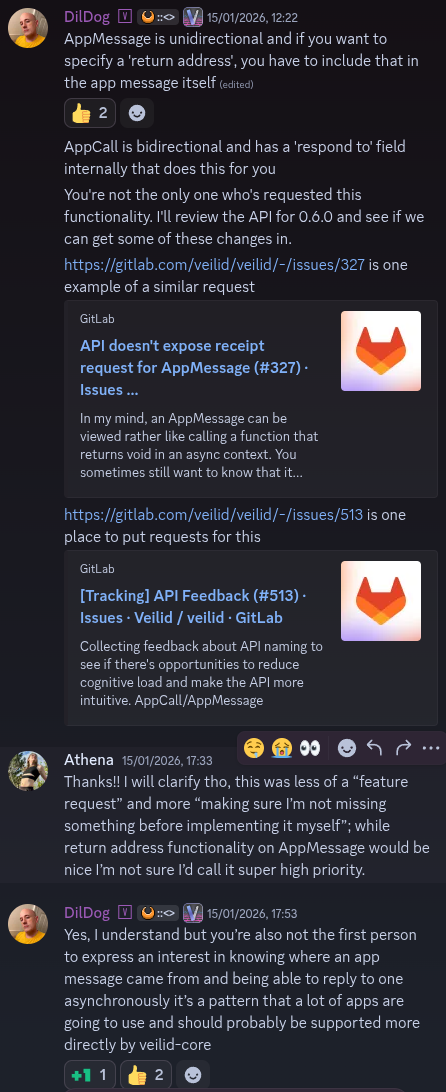
\includegraphics[width=\textwidth,height=0.8\textheight,keepaspectratio]{Figures/screenshots/veilid2.png}
\caption{Discussion of \texttt{app\_call} vs.\ \texttt{app\_message}
  semantics: \texttt{app\_call} is bidirectional with a response, while
  \texttt{app\_message} is fire-and-forget with no delivery guarantee.}
\label{fig:veilid-discord-2}
\end{figure}

\begin{figure}[H]
\centering
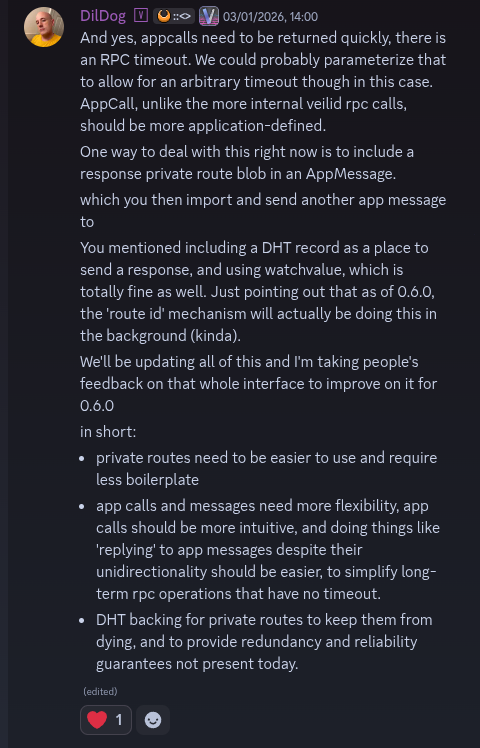
\includegraphics[width=0.7\textwidth]{Figures/screenshots/veilid3.png}
\caption{DilDog on planned improvements to the Veilid API: private route
  resilience, provider routing, and DHT publishing of route blobs.}
\label{fig:veilid-discord-3}
\end{figure}

\begin{figure}[H]
\centering

\includegraphics[width=0.7\textwidth]{Figures/screenshots/veilid4.png}
\caption{DilDog on DHT record design patterns: using subkey~0 as a header
  for eventually consistent updates, and the relationship to CRDTs.}
\label{fig:veilid-discord-4}
\end{figure}

\begin{figure}[H]
\centering
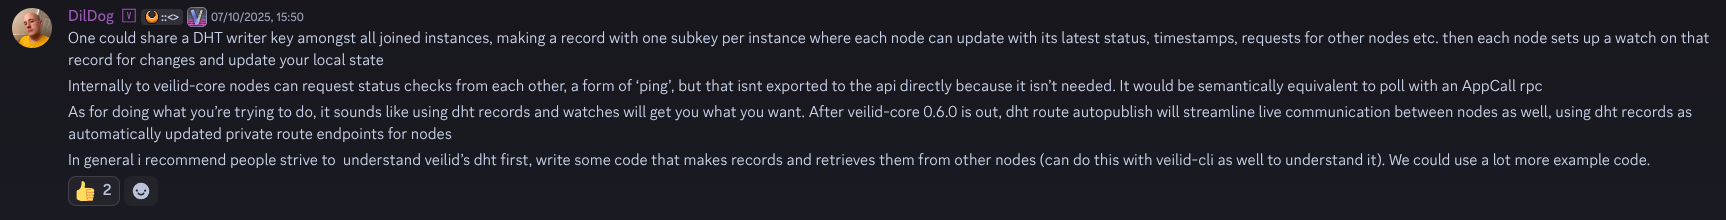
\includegraphics[width=\textwidth]{Figures/screenshots/veilid5.png}
\caption{DilDog on DHT record ownership and multi-writer patterns: each
  node can own a record and update its subkeys independently, with
  eventual consistency across the network.}
\label{fig:veilid-discord-5}
\end{figure}

\end{document}

